\documentclass{ieeeaccess}
\usepackage[utf8]{inputenc}
\usepackage{cite}
\usepackage{amsmath,amssymb,amsfonts}
\usepackage{graphicx}
\usepackage{textcomp}
\usepackage{booktabs}
\usepackage{microtype}
\usepackage{ragged2e}
\usepackage{tikz}
\usetikzlibrary{arrows.meta, positioning, fit, backgrounds, calc}
\usepackage[portuguese]{babel}
\addto\captionsportuguese{\renewcommand{\refname}{References}}

% [FIX] O tikz carrega o xcolor, que quebra o spot color PANTONE "accessblue"
% da classe (Incompatible color definition). Sem ele, o TÍTULO e os rótulos
% azuis ABSTRACT / INDEX TERMS ficam invisíveis. Redefinimos accessblue com o
% mesmo CMYK do PANTONE 3015 C que a própria classe usa (linha AddSpotColor).
\definecolor{accessblue}{cmyk}{1,0.3,0,0.2}

% Paleta em tons de cinza + destaque para os diagramas de blocos
\definecolor{blkBase}{RGB}{237,237,237}   % cinza claro (blocos comuns)
\definecolor{blkEdge}{RGB}{120,120,120}   % borda cinza
\definecolor{blkHi}{RGB}{196,210,225}     % destaque (azul-ardósia dessaturado)
\definecolor{blkHiEdge}{RGB}{82,110,143}  % borda do destaque

\usepackage{bm}
\makeatletter
\AtBeginDocument{\DeclareMathVersion{bold}
\SetSymbolFont{operators}{bold}{T1}{times}{b}{n}
\SetSymbolFont{NewLetters}{bold}{T1}{times}{b}{it}
\SetMathAlphabet{\mathrm}{bold}{T1}{times}{b}{n}
\SetMathAlphabet{\mathit}{bold}{T1}{times}{b}{it}
\SetMathAlphabet{\mathbf}{bold}{T1}{times}{b}{n}
\SetMathAlphabet{\mathtt}{bold}{OT1}{pcr}{b}{n}
\SetSymbolFont{symbols}{bold}{OMS}{cmsy}{b}{n}
\renewcommand\boldmath{\@nomath\boldmath\mathversion{bold}}}
\makeatother

\graphicspath{{images/}}

\setlength{\emergencystretch}{3em}

\def\BibTeX{{\rm B\kern-.05em{\sc i\kern-.025em b}\kern-.08em
    T\kern-.1667em\lower.7ex\hbox{E}\kern-.125emX}}

\begin{document}
\history{}
\doi{}

\title{Identificação de Sistema e Modelagem de um Veículo Aéreo Não Tripulado (VANT) VTOL Híbrido no Modo Quadricóptero}

\author{\uppercase{Henrique Mark dos Santos Corrêa}\authorrefmark{1} and
\uppercase{Neusa Maria Franco de Oliveira}\authorrefmark{1}}

\address[1]{Departamento de Engenharia Eletrônica (IEE), Instituto Tecnológico de Aeronáutica (ITA), São José dos Campos, SP 12228-900, Brazil (e-mail: henriquecorrea@ita.br; neusa@ita.br)}

\tfootnote{Trabalho desenvolvido no âmbito do programa de pós-graduação em Engenharia Eletrônica e Computação do Instituto Tecnológico de Aeronáutica (ITA).}

\markboth
{Corrêa \MakeLowercase{\textit{et al.}}: Identificação de Sistema e Modelagem de um VANT VTOL Híbrido no Modo Quadricóptero}
{Corrêa \MakeLowercase{\textit{et al.}}: Identificação de Sistema e Modelagem de um VANT VTOL Híbrido no Modo Quadricóptero}

\corresp{Corresponding author: Henrique Mark dos Santos Corrêa (e-mail: henriquecorrea@ita.br).}

\begin{abstract}
O presente trabalho descreve a identificação de sistema e a validação de um modelo matemático não-linear para o modo de voo quadricóptero de um Veículo Aéreo Não Tripulado (VANT) VTOL de configuração híbrida. O objetivo principal é obter um modelo identificado do modo quadricóptero que sirva como base para o desenvolvimento de algoritmos de controle e de um piloto automático (PA) para as fases de decolagem e pouso vertical. A metodologia de identificação de sistemas M4V (Maneuver, Measurements, Methods, Models) foi aplicada, utilizando dados coletados em voos reais. Para estimar os parâmetros de inércia e os coeficientes aerodinâmicos, empregou-se um método de otimização por mínimos quadrados não-lineares no domínio do tempo, que minimiza o erro entre a resposta simulada e os dados medidos em manobras que excitaram os modos da aeronave. O modelo identificado foi validado comparando-se suas respostas com um conjunto distinto de dados de voo não utilizado na estimação. Os resultados demonstram boa correlação entre os dados reais e simulados, confirmando a adequação do modelo para as aplicações de controle pretendidas.
\end{abstract}

\begin{keywords}
Identificação de sistemas, método do erro de saída (OEM), modelagem dinâmica, modo quadricóptero, VANT VTOL híbrido.
\end{keywords}

\titlepgskip=-21pt

\maketitle

\section{Introdução}
\label{sec:introducao}

\PARstart{V}{eículos} aéreos não tripulados (VANTs) com capacidade de decolagem e pouso vertical (VTOL, do inglês \textit{Vertical Take-off and Landing}) têm ganhado destaque devido à sua versatilidade, combinando a eficiência de cruzeiro de uma aeronave de asa fixa com a flexibilidade operacional de um multirotor~\cite{c1}. A aeronave objeto deste estudo, o DH Hybrid-Drone VTOL, é um VANT de configuração híbrida capaz de transitar entre o modo de voo quadricóptero e o modo de asa fixa. A Figura~\ref{fig:fases_voo} ilustra as fases típicas de voo desse tipo de aeronave, desde a decolagem vertical até o pouso, passando pela transição e pelo cruzeiro como asa fixa.

Embora a aeronave opere em múltiplos modos de voo, as fases de decolagem e pouso vertical são realizadas exclusivamente no modo quadricóptero e constituem uma etapa importante para a operação autônoma. Nesse contexto, o presente trabalho concentra-se na identificação do modelo dinâmico do modo quadricóptero, levando em consideração as particularidades de uma plataforma VTOL híbrida como, por exemplo, a distribuição de massa assimétrica decorrente da configuração H-frame e influência nos momentos de inércia da aeronave.

\begin{figure}[!htbp]
      \centering
      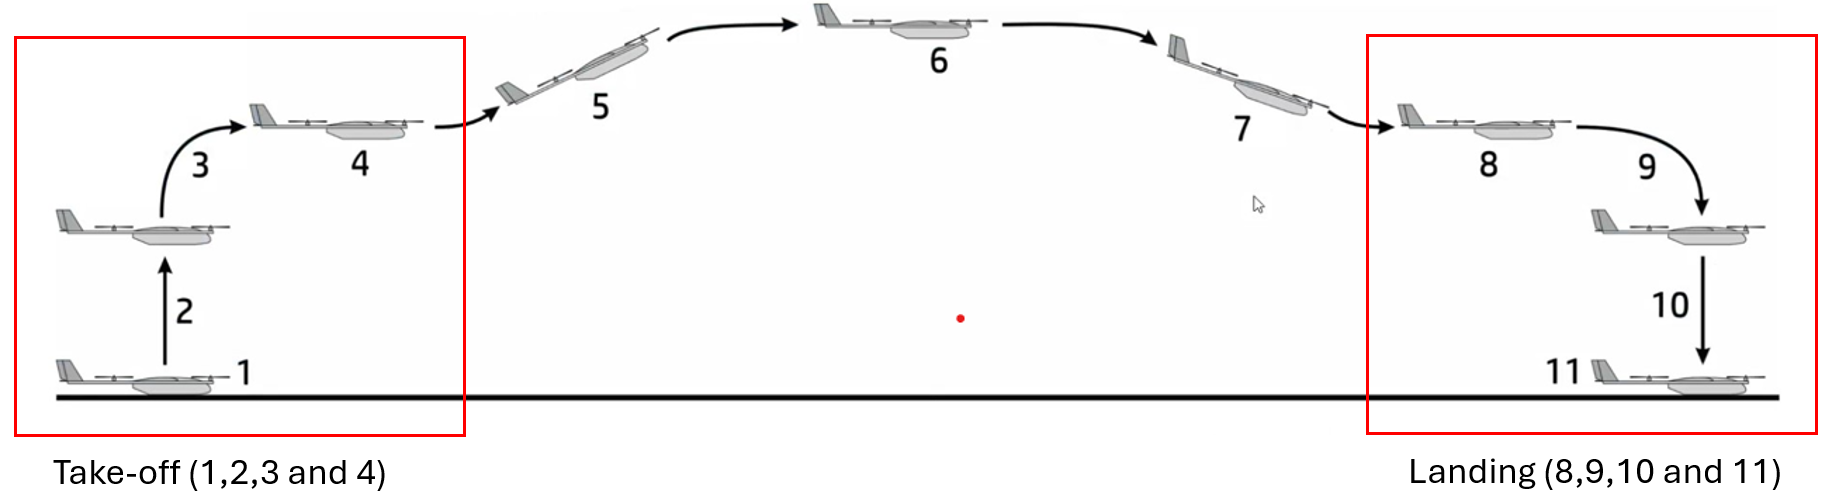
\includegraphics[width=\columnwidth]{passos.png}
      \caption{Ilustração das etapas de voo de um VTOL híbrido.}
      \label{fig:fases_voo}
\end{figure}

O objetivo principal é obter, a partir de dados de voo reais, um modelo matemático não-linear identificado que represente com fidelidade a dinâmica do modo quadricóptero. Esse modelo servirá como base para o desenvolvimento de algoritmos de controle e de um piloto automático (PA) para as manobras autônomas de decolagem e pouso vertical. A identificação é realizada a partir de valores iniciais obtidos da caracterização dos motores com as curvas de empuxo e contra-torque dos motores obtidas em bancada, dos momentos de inércia da aeronave obtidos em softwares de simulação e de dados coletados em manobras de voo específicas.

\section{Método M4V de Identificação}
\label{sec:m4v}

Para a identificação do sistema, foi utilizada a metodologia M4V (Maneuver, Measurements, Methods, Models, Validation), uma abordagem estruturada e amplamente utilizada na identificação de sistemas de veículos aéreos~\cite{c2}. A metodologia M4V divide o processo de identificação em fases bem definidas, garantindo uma abordagem sistemática e robusta.

\begin{figure}[!htbp]
      \centering
      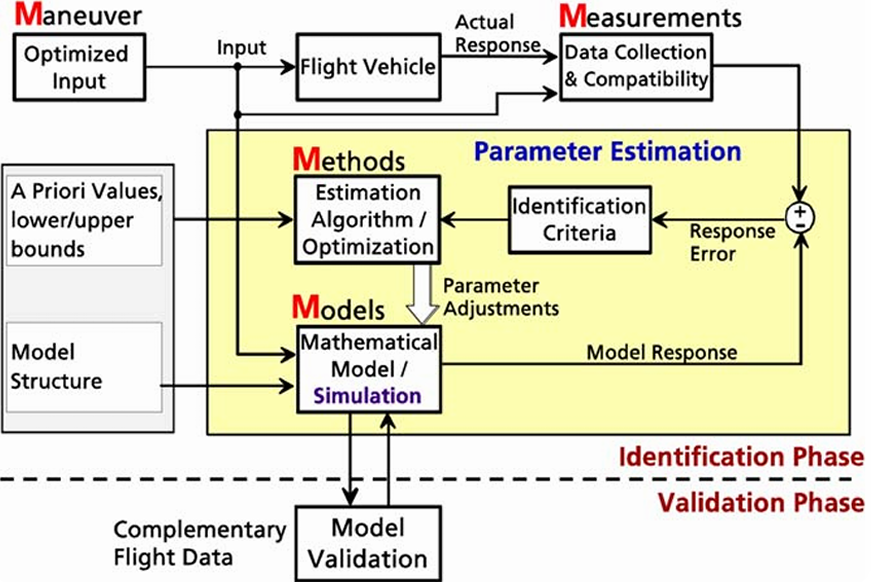
\includegraphics[width=\columnwidth]{m4m.png}
      \caption{Diagrama do método M4V.}
      \label{fig:m4v}
\end{figure}

\begin{RaggedRight}
As fases da metodologia M4V são:
\begin{itemize}
    \item \textbf{Maneuver (Manobra):} Entradas otimizadas são projetadas e aplicadas ao veículo em voo para excitar adequadamente a sua dinâmica.
    \item \textbf{Measurements (Medições):} Os dados da resposta real da aeronave às manobras são coletados por meio de sensores embarcados. A compatibilidade e a qualidade dos dados são verificadas nesta fase.
    \item \textbf{Methods (Métodos):} Algoritmos de estimação e otimização são utilizados para identificar os parâmetros do modelo matemático. O ajuste é feito com base em critérios de identificação, em particular na minimização do erro entre resposta real e simulada.
    \item \textbf{Models (Modelos):} Um modelo matemático estrutural, com valores iniciais (a priori), é continuamente refinado com os parâmetros estimados até que o erro seja minimizado.
\end{itemize}
\end{RaggedRight}

Após a fase de identificação, o modelo obtido é submetido a uma fase de validação, na qual dados de voo complementares, não utilizados na estimação, são usados para verificar a capacidade preditiva e a robustez do modelo.

\section{Modelo Matemático do Modo Quadricóptero}
\label{sec:modelo}

O modelo matemático foi desenvolvido considerando a aeronave como um corpo rígido 6-DOF operando no modo quadricóptero. Neste modo, a sustentação e o controle de atitude são realizados exclusivamente pelos quatro motores verticais, enquanto o motor traseiro de cruzeiro e as superfícies aerodinâmicas permanecem inativos. Embora a configuração VTOL híbrida introduza particularidades na distribuição de massa e na geometria da aeronave em relação a um quadricóptero convencional, a dinâmica neste modo é governada unicamente pelas forças e momentos gerados pelos rotores verticais. As Figuras~\ref{fig:drone_config} e~\ref{fig:drone_real} ilustram a disposição dos motores, com os momentos e as forças por eles aplicados na aeronave.

\begin{figure}[!htbp]
      \centering
      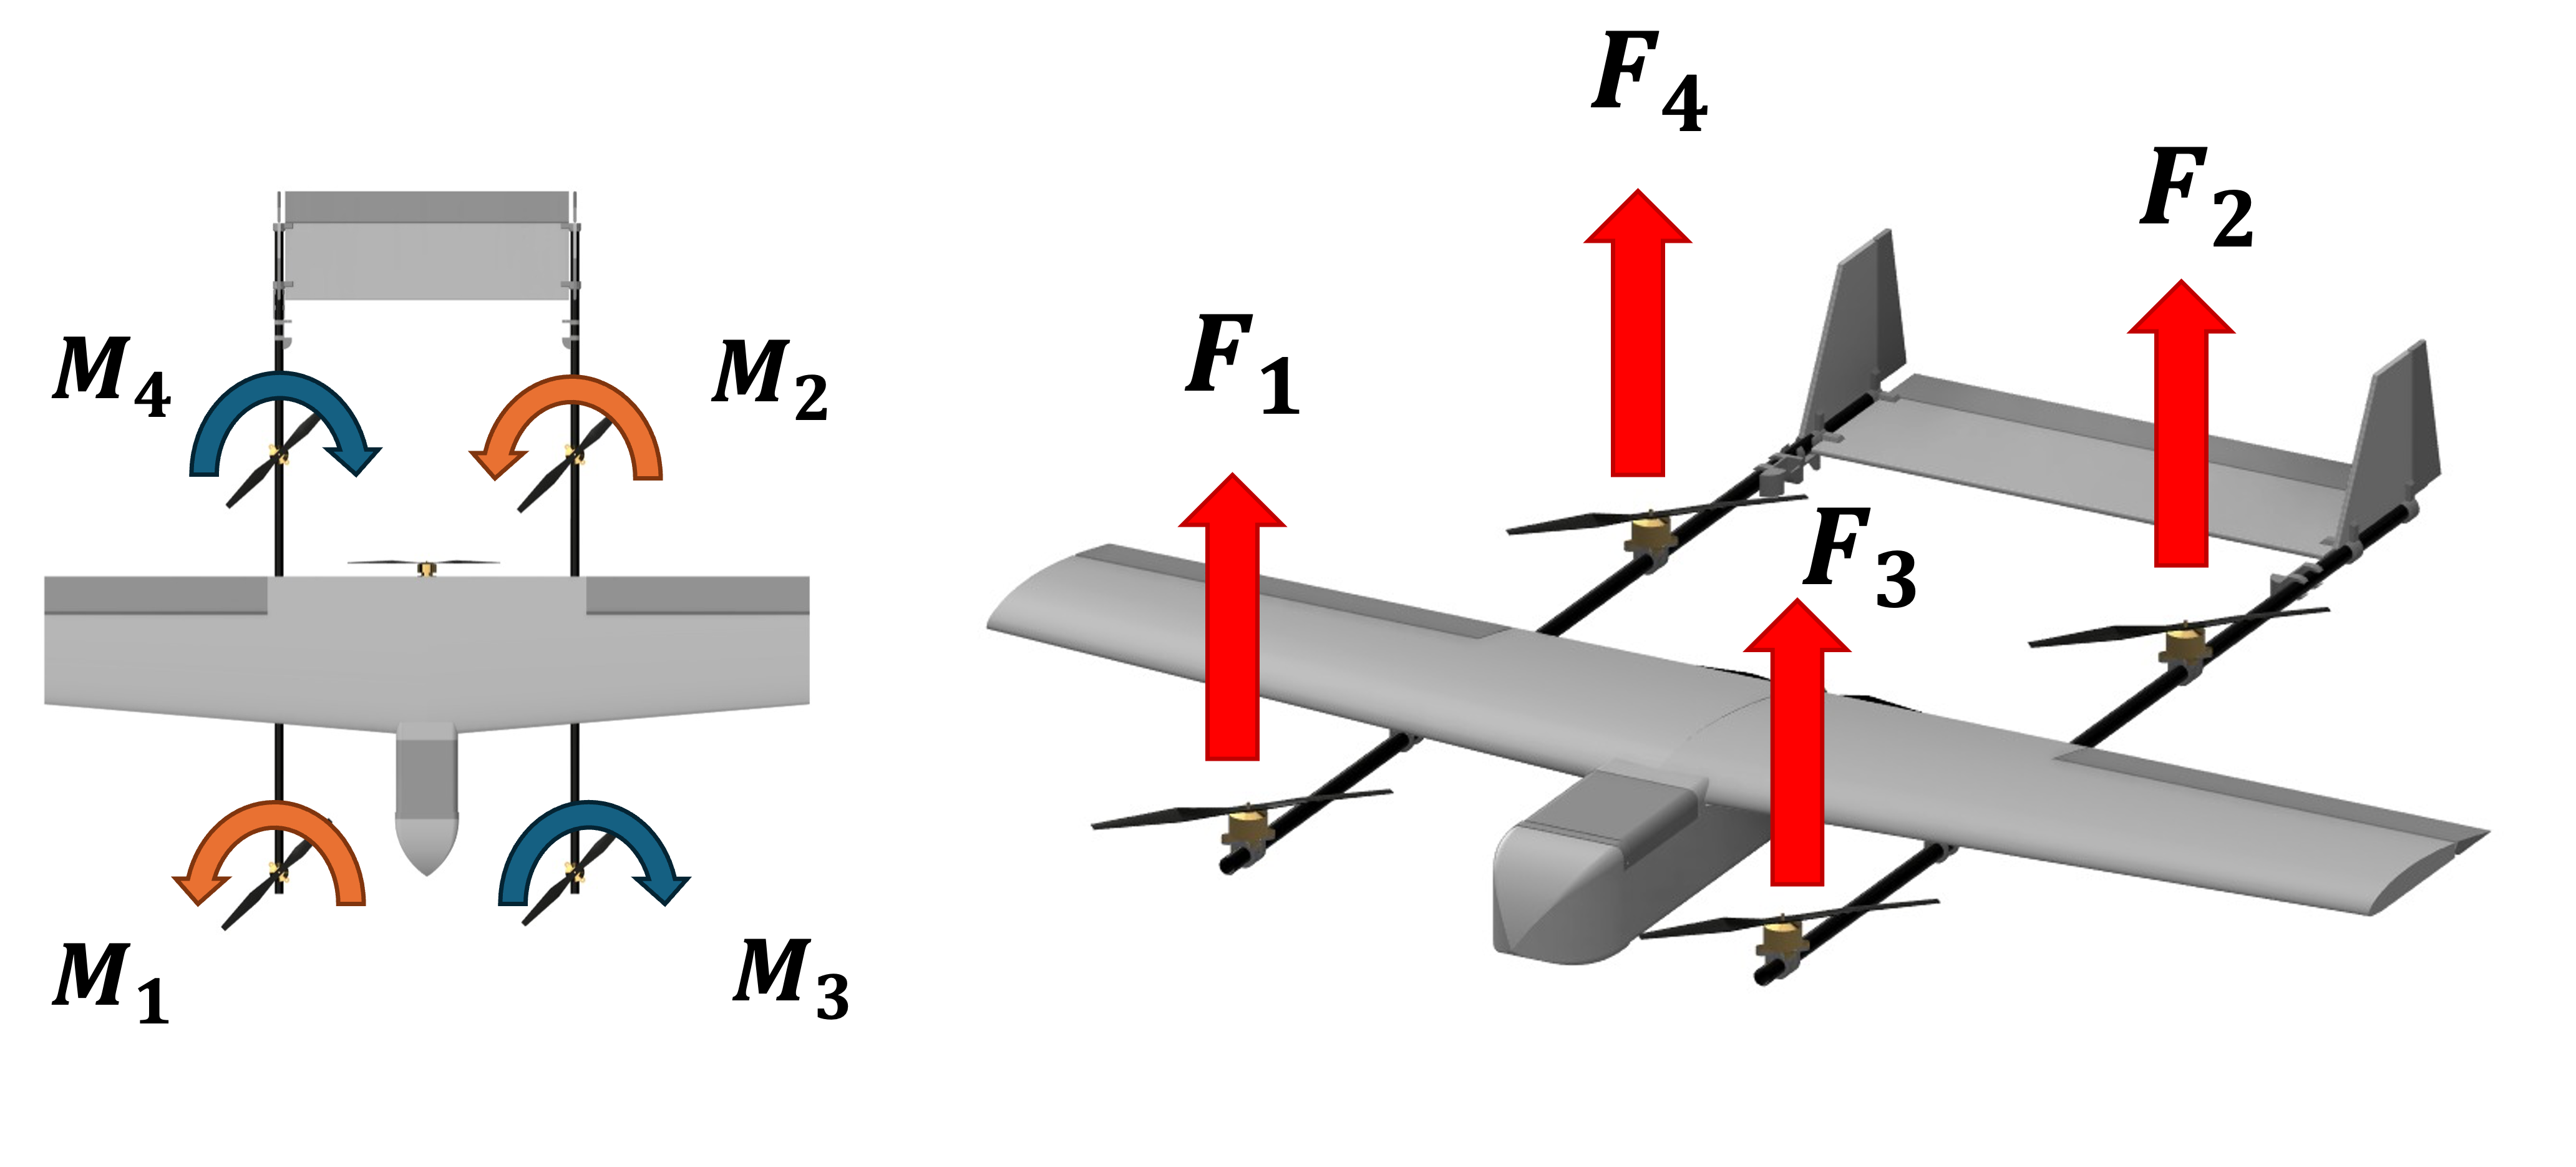
\includegraphics[width=\columnwidth]{forcas-momentos.png}
      \caption{Relação de momentos e forças aplicados pelos motores.}
      \label{fig:drone_config}
\end{figure}

\begin{figure}[!htbp]
      \centering
      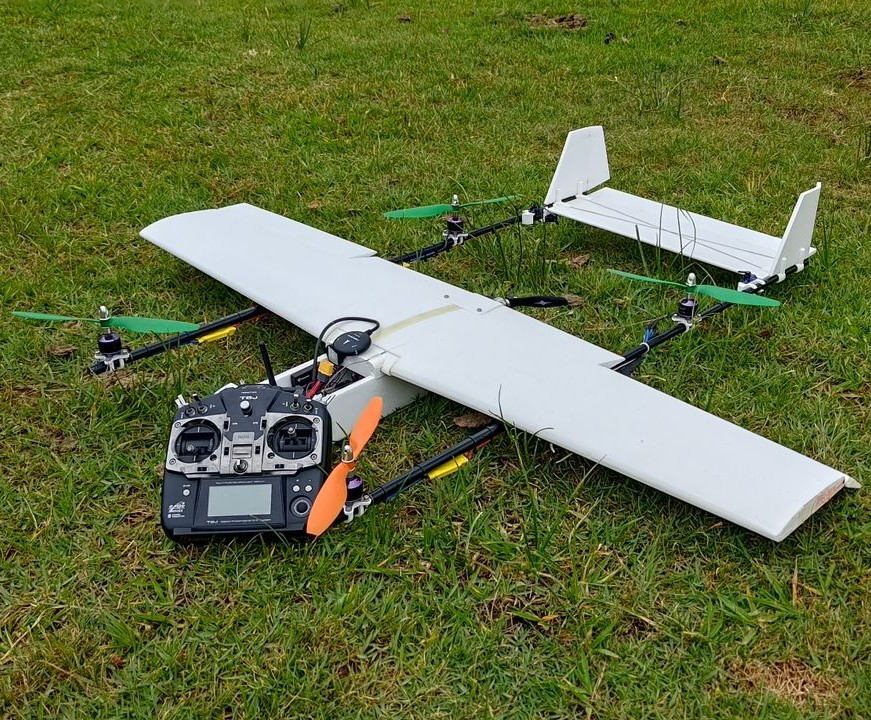
\includegraphics[width=\columnwidth]{rdrone.jpeg}
      \caption{Aeronave DH Hybrid-Drone VTOL.}
      \label{fig:drone_real}
\end{figure}

O modelo é descrito por um conjunto de equações de estado não-lineares. Os vetores de estado $\mathbf{x}$ e de entrada $\mathbf{u}$ são definidos como:
\begin{equation}
    \mathbf{x} = [\phi, \theta, \psi, p, q, r, u, v, w]^T
\end{equation}
\begin{equation}
    \mathbf{u} = [\sigma_1, \sigma_2, \sigma_3, \sigma_4]^T
\end{equation}
Onde $\phi, \theta, \psi$ são os ângulos de Euler (rolagem, arfagem e guinada); $p, q, r$ são as velocidades angulares no referencial do corpo; $u, v, w$ são as velocidades lineares no sistema de eixos do corpo; e $\sigma_i$ são os comandos de PWM normalizados enviados aos quatro motores do multirotor~\cite{c3}, detalhados a seguir no modelo do motor.

Este modelo matemático completo é dividido em três partes: primeiro o modelo dos motores e a geração agregada das forças e momentos instantâneos, em seguida a dinâmica do corpo rígido que é separada em modelo rotacional e modelo translacional. A Figura~\ref{fig:model_diagram} resume essa estrutura em blocos, do comando dos motores às saídas da dinâmica do corpo rígido.

\begin{figure}[!t]
\centering
\resizebox{\columnwidth}{!}{%
\begin{tikzpicture}[
    sysblock/.style={rectangle, draw=blkEdge, semithick, fill=blkBase, rounded corners=3pt, minimum height=1.4cm, text width=2.2cm, align=center, font=\footnotesize},
    hi/.style={fill=blkHi, draw=blkHiEdge, thick},
    io/.style={font=\footnotesize},
    arr/.style={-{Stealth[length=2.5mm]}, semithick, black!62},
    darr/.style={-{Stealth[length=2.5mm]}, semithick, black!48, dashed},
    lbl/.style={font=\scriptsize, fill=white, inner sep=1.5pt, text=black!80},
    dot/.style={circle, fill=black!62, inner sep=0pt, minimum size=4pt},
]

% ========== ROW 1 (y=0): sigma (PWM) -> Modelo do Motor -> (T_i,Q_i) -> B -> RotDyn ==========
\node[io, align=center] at (0,0) (sig) {$\sigma_i$\\(PWM)};
\node[sysblock, hi, text width=1.9cm] at (2.7,0) (motor) {Modelo do\\Motor};
\node[sysblock, text width=1.8cm] at (5.5,0) (balloc) {Matriz de\\alocação $\mathbf{B}$};
\node[sysblock, hi] at (8.3,0) (rotdyn) {Dinâmica\\Rotacional\\$\dot{p},\dot{q},\dot{r}$};

\draw[arr] (sig) -- (motor);
\draw[arr] ([yshift=0.22cm]motor.east) -- node[lbl, above] {$T_i$} ([yshift=0.22cm]balloc.west);
\draw[arr] ([yshift=-0.22cm]motor.east) -- node[lbl, below] {$Q_i$} ([yshift=-0.22cm]balloc.west);
\draw[arr] (balloc) -- node[lbl, above] {$\tau_x,\tau_y,\tau_z$} (rotdyn);

% Output p,q,r
\node[io] at (10.6,0) (pqr_out) {$p, q, r$};
\draw[arr] (rotdyn) -- (pqr_out);

% ========== ROW 2 (y=-4): Euler ==========
\node[sysblock] at (8.3,-4) (euler) {Cinemática\\de Euler\\$\dot{\phi},\dot{\theta},\dot{\psi}$};
\node[io] at (10.6,-4) (att_out) {$\phi, \theta, \psi$};
\draw[arr] (euler) -- (att_out);

% ========== ROW 3 (y=-8): TransDyn ==========
\node[sysblock, hi] at (8.3,-8) (transdyn) {Dinâmica\\Translacional\\$\dot{u},\dot{v},\dot{w}$};
\node[io] at (10.6,-7.7) (uvw_out) {$u, v, w$};
\node[io] at (10.6,-8.3) (acc_out) {$\dot{u}, \dot{v}, \dot{w}$};
\draw[arr] ([yshift=0.3cm]transdyn.east) -- (uvw_out);
\draw[arr] ([yshift=-0.3cm]transdyn.east) -- (acc_out);

% m, g input (enters bottom of west side)
\node[io] at (6.1,-8.35) (const) {$m, g$};
\draw[arr] (const) -- ([yshift=-0.35cm]transdyn.west);

% ========== CONNECTIONS ==========

% --- Empuxo total T: B -> TransDyn (solid, down, enters west middle) ---
\draw[arr] (balloc.south) -- (5.5,-8.0) -- node[lbl, above] {$T$} ([yshift=0.0cm]transdyn.west);

% --- RotDyn -> Euler (solid, center vertical) ---
\node[dot] at (8.3,-1.5) (junc) {};
\draw[semithick, black!62] (rotdyn.south) -- (junc);
\draw[arr] (junc) -- node[lbl, left] {$p,q,r$} (euler.north);

% --- p,q,r -> TransDyn (dashed, enters west top) ---
\draw[darr] (junc.west) -- (6.9,-1.5) -- (6.9,-7.65) -- ([yshift=0.35cm]transdyn.west);

% --- Euler -> TransDyn (solid, center) ---
\draw[arr] (euler.south) -- node[lbl, left] {$\phi,\theta,\psi$} (transdyn.north);

\end{tikzpicture}%
}
\caption{Diagrama de blocos do modelo dinâmico do DH com os três subsistemas: Modelo do Motor, Modelo Rotacional e Modelo Translacional}
\label{fig:model_diagram}
\end{figure}

\subsection{Modelo do Motor}

O modelo do motor descreve a cadeia que converte o comando de PWM aplicado em cada motor nos esforços generalizados aplicados ao corpo rígido. Inicialmente o comando PWM normalizado $\sigma_i$ é convertido em velocidade angular do rotor $\Omega_i$, o qual produz o empuxo $T_i$ e o contra-torque $Q_i$, então esses esforços individuais são, por fim, combinados pela matriz de alocação $\mathbf{B}$ no empuxo total $T$ e nos momentos $\tau_x$, $\tau_y$ e $\tau_z$~\cite{c13}. A Figura~\ref{fig:blocos_motor} apresenta a estrutura em dois estágios desse modelo incluindo a dinâmica de primeira ordem, que modela o atraso na resposta do motor. 

Os valores tanto de entrada como saída foram obtidos a partir de ensaios em uma bancada dinamométrica, o qual relacionava o comando de entrada com a velocidade angular do rotor, empuxo e contra-torque gerado com a hélice acoplada, ambos com a bateria carregada para descosiderar os efeitos da perda de potência, simplificando a análise.

\begin{figure}[!htbp]
      \centering
      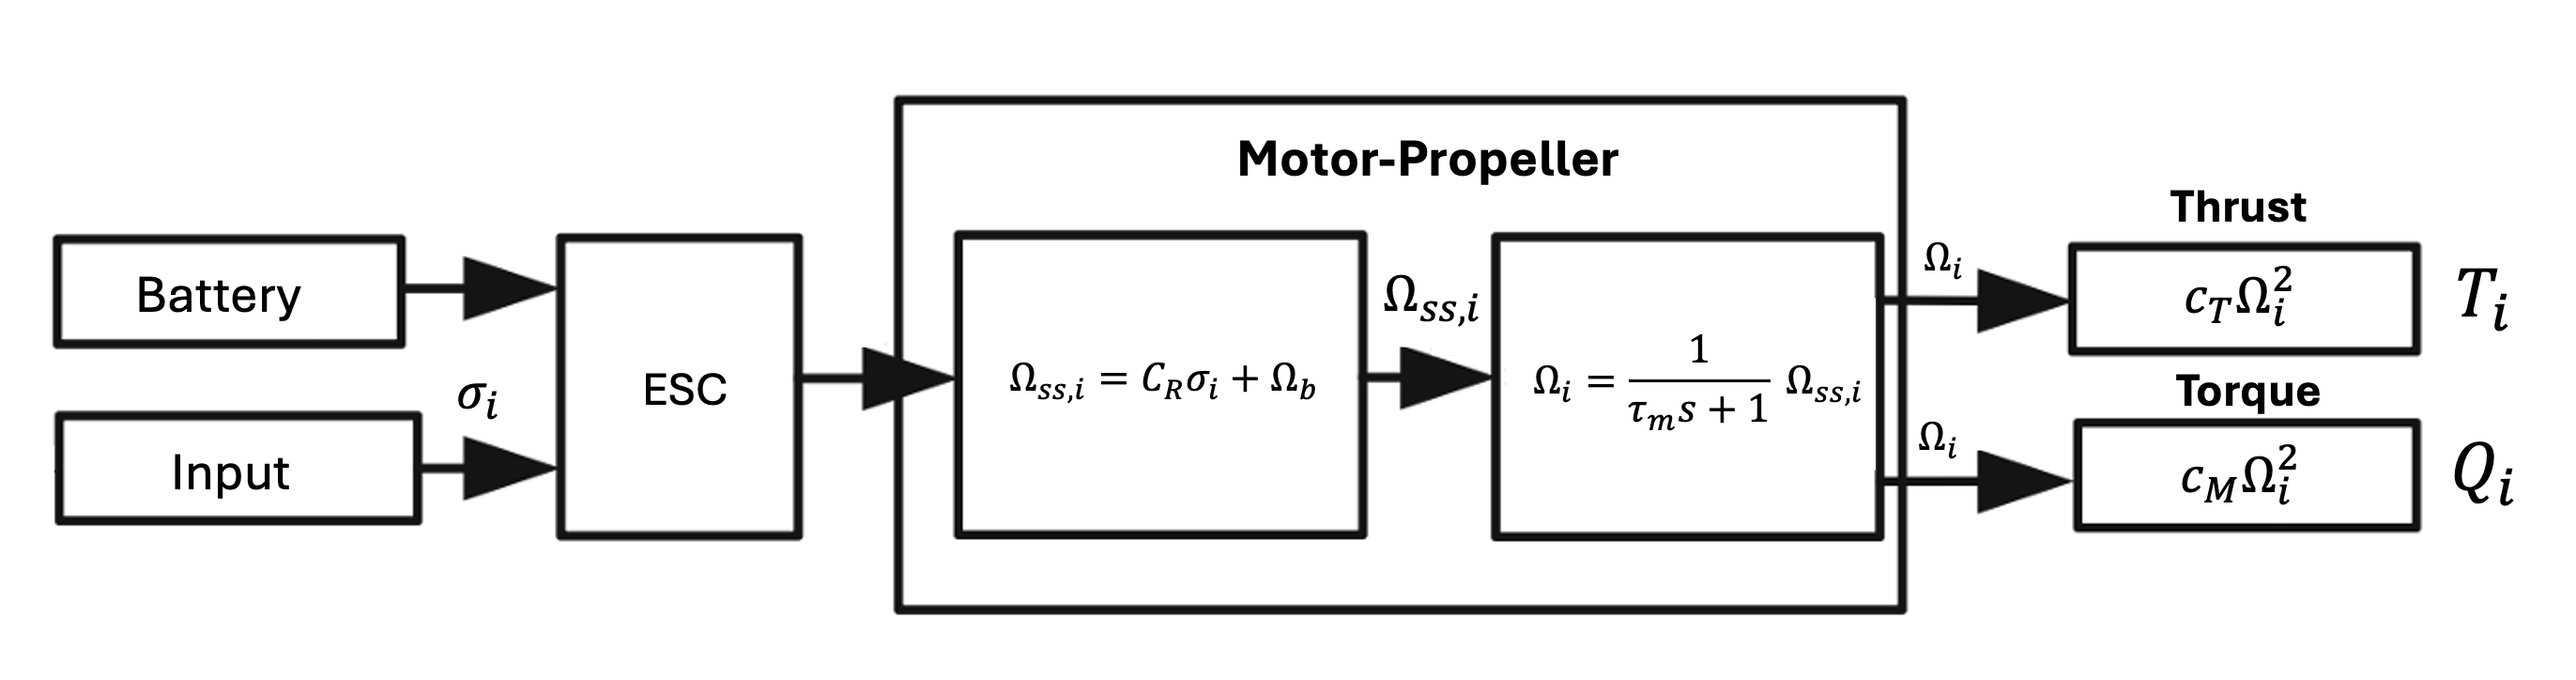
\includegraphics[width=\columnwidth]{blocos-motor.png}
      \caption{Diagrama de blocos do modelo do motor: o ESC converte o comando normalizado $\sigma_i$ em velocidade angular de regime permanente (Equação~\eqref{eq:omega-ss}), filtrada pela dinâmica de primeira ordem (Equação~\eqref{eq:omega-lag}) e transformada em empuxo e contra-torque (Equação~\eqref{eq:tq}). Adaptado de~\cite{c13}.}
      \label{fig:blocos_motor}
\end{figure}

O comando de cada motor é a largura de pulso $\delta_{PWM,i}$, normalizada para o intervalo $[0,1]$:
\begin{equation}
\sigma_i = \frac{\delta_{PWM,i} - \delta_{\min}}{\delta_{\max} - \delta_{\min}}
\label{eq:norm}
\end{equation}
em que $\delta_{\min} = 1000~\mu$s e $\delta_{\max} = 2000~\mu$s são os limites da faixa de operação do ESC.

A primeira etapa da cadeia relaciona o comando normalizado com a velocidade angular do rotor. Em regime permanente, os dados de bancada da Figura~\ref{fig:motor_pwm_rpm} mostram que essa relação é bem aproximada por uma reta~\cite{c13}:
\begin{equation}
\Omega_{ss,i} = C_R\,\sigma_i + \Omega_b
\label{eq:omega-ss}
\end{equation}
onde $C_R$ é o ganho do conjunto ESC--motor e $\Omega_b$ é a velocidade angular mínima de operação. O ajuste por mínimos quadrados aos pontos medidos, excluindo o ponto de motor parado, resulta em $C_R = 4523$~RPM e $\Omega_b = 1837$~RPM.

\begin{figure}[!htbp]
      \centering
      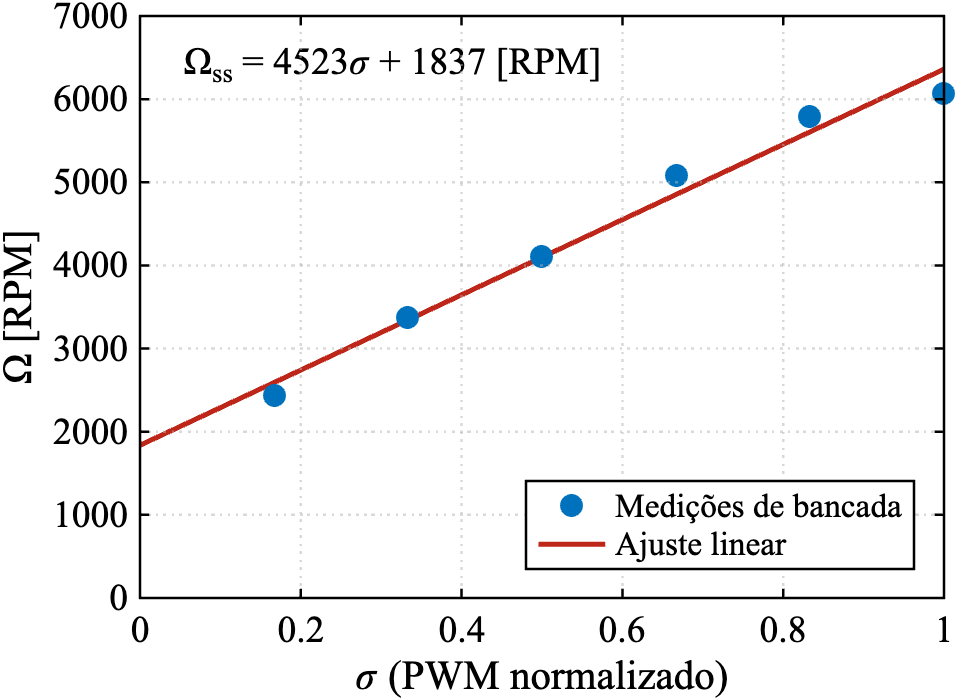
\includegraphics[width=\columnwidth]{motor_pwm_rpm.png}
      \caption{Velocidade angular do rotor em regime permanente em função do comando PWM normalizado. Os pontos são as medições de bancada e a linha contínua é o ajuste linear da Equação~\eqref{eq:omega-ss}.}
      \label{fig:motor_pwm_rpm}
\end{figure}

Porém, a resposta do conjunto ESC--motor--hélice não é instantânea: a velocidade angular converge para o valor de regime com uma dinâmica bem aproximada por um sistema de primeira ordem que, no domínio da frequência, corresponde a um filtro passa-baixas~\cite{c13}:
\begin{equation}
\Omega_i(s) = \frac{1}{\tau_m s + 1}\,\Omega_{ss,i}(s)
\label{eq:omega-lag}
\end{equation}
em que $s$ é a variável de Laplace e $\tau_m = 0{,}05$~s é a constante de tempo adotada. A velocidade angular instantânea $\Omega_i$ resultante dessa dinâmica é a grandeza que efetivamente gera os esforços do rotor.

Cada rotor, girando com velocidade $\Omega_i$, produz um empuxo e um contra-torque proporcionais ao quadrado dessa velocidade~\cite{c11},~\cite{c13}:
\begin{equation}
T_i = c_{T_i}\,\Omega_i^{2}, \qquad Q_i = c_{M_i}\,\Omega_i^{2}
\label{eq:tq}
\end{equation}
onde $c_{T_i}$ e $c_{M_i}$ são os coeficientes de empuxo e de torque, dependentes da geometria da hélice e da densidade do ar, tratados como parâmetros identificáveis do modelo. O ajuste quadrático aos dados de bancada, apresentado na Figura~\ref{fig:motor_tq}, fornece os valores de referência $c_T = 1{,}76\times10^{-7}$~N/RPM$^2$ e $c_M = 5{,}04\times10^{-9}$~N$\cdot$m/RPM$^2$, adotados como valores iniciais do processo de identificação (Tabela~\ref{tab:const_iniciais}), no qual são refinados individualmente para cada motor.

\begin{figure}[!htbp]
      \centering
      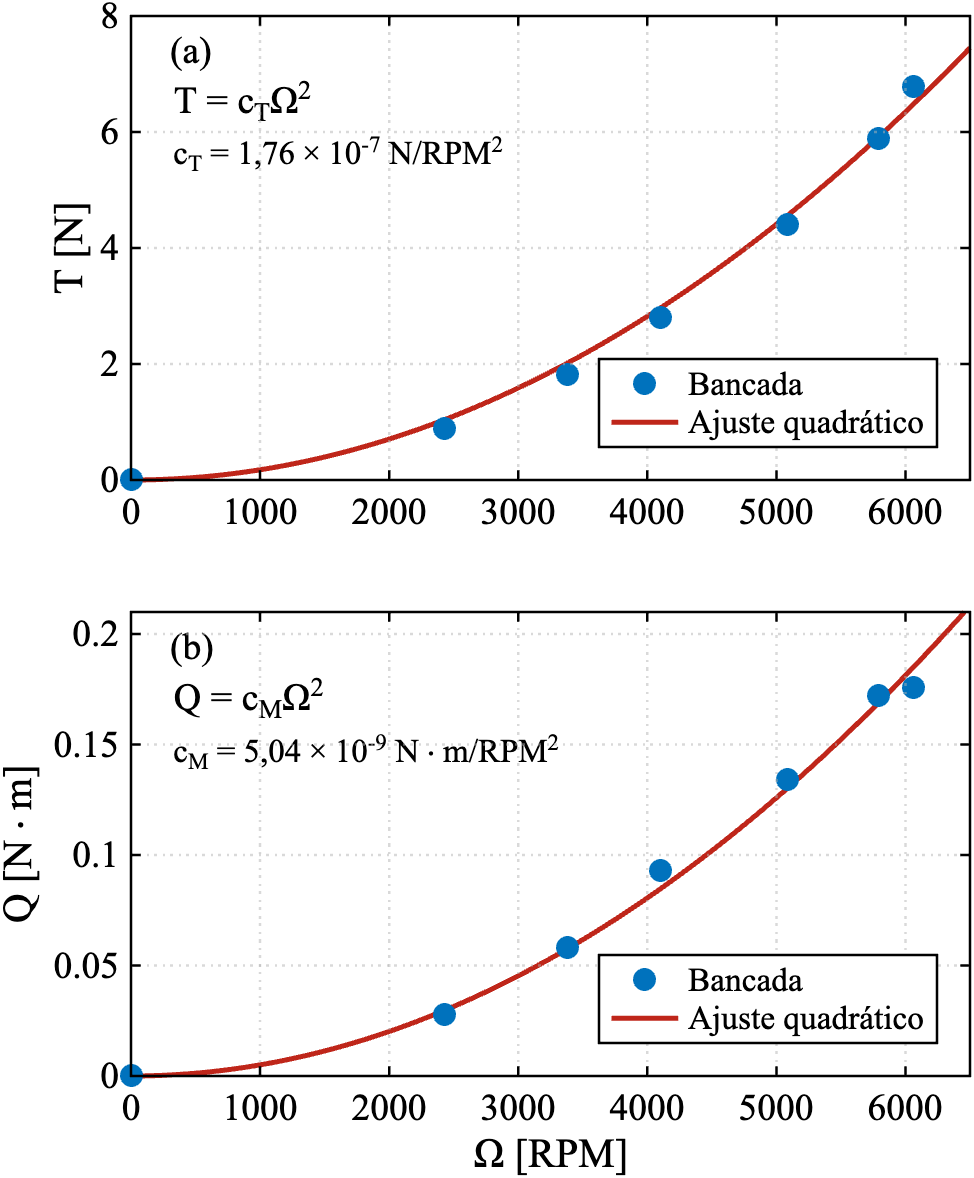
\includegraphics[width=\columnwidth]{motor_thrust_torque.png}
      \caption{Empuxo (a) e contra-torque (b) em função da velocidade angular do rotor. Os pontos são as medições de bancada e as linhas contínuas são os ajustes quadráticos da Equação~\eqref{eq:tq}.}
      \label{fig:motor_tq}
\end{figure}

Os esforços individuais combinam-se em função da geometria da aeronave. Os momentos de rolagem e arfagem resultam do empuxo diferencial dos motores, ponderado pelas distâncias de cada rotor ao centro de gravidade: $L_{x_r}$ e $L_{x_l}$ são os braços laterais dos rotores dos lados direito (motores 1 e 4) e esquerdo (motores 2 e 3), e $L_{y_f}$ e $L_{y_r}$ são os braços longitudinais dos rotores dianteiros (motores 1 e 3) e traseiros (motores 2 e 4), distintos entre si na configuração H-frame. O momento de guinada, por sua vez, é gerado pelo contra-torque das hélices: os motores 1 e 2 giram em um sentido e os motores 3 e 4 no sentido oposto, de modo a cancelar o torque resultante em voo pairado~\cite{c5}. Da Equação~\eqref{eq:tq} obtém-se a relação entre o contra-torque e o empuxo de cada rotor:
\begin{equation}
Q_i = \frac{c_M}{c_T}\,T_i
\label{eq:qt-ratio}
\end{equation}
que permite expressar os contra-torques em função dos empuxos, reunindo todas as contribuições em uma única matriz de alocação $\mathbf{B}$:
\begin{equation}
\begin{bmatrix} T \\ \tau_x \\ \tau_y \\ \tau_z \end{bmatrix}
=
\underbrace{\begin{bmatrix}
1 & 1 & 1 & 1 \\
-L_{x_r} & L_{x_l} & L_{x_l} & -L_{x_r} \\
L_{y_f} & -L_{y_r} & L_{y_f} & -L_{y_r} \\
\tfrac{c_M}{c_T} & \tfrac{c_M}{c_T} & -\tfrac{c_M}{c_T} & -\tfrac{c_M}{c_T}
\end{bmatrix}}_{\mathbf{B}}
\begin{bmatrix} T_1 \\ T_2 \\ T_3 \\ T_4 \end{bmatrix}
\label{eq:aloca}
\end{equation}

O modelo do motor estabelece, assim, o caminho completo das medidas de bancada ao modelo dinâmico: dos pares PWM--velocidade angular obtém-se $C_R$; dos pares velocidade angular--empuxo e velocidade angular--contra-torque obtêm-se $c_T$ e $c_M$, que geram os empuxos $T_1$ a $T_4$; e a matriz de alocação converte esses empuxos no empuxo total $T$, que alimenta o modelo translacional, e nos momentos $\tau_x$, $\tau_y$ e $\tau_z$, que alimentam o modelo rotacional.

\subsection{Modelo Rotacional}

O modelo rotacional deriva da segunda lei de Newton para a rotação, que iguala a taxa de variação do momento angular $\mathbf{h}$ à soma dos momentos aplicados ao corpo $\boldsymbol{\tau}$~\cite{cBeard}:
\begin{equation}
\frac{d\mathbf{h}}{dt} = \boldsymbol{\tau}
\label{eq:rot-newton}
\end{equation}
Expressa no referencial do corpo, com $\mathbf{h} = \mathbf{J}\boldsymbol{\omega}$ e aplicando o teorema do transporte, isola-se a aceleração angular $\dot{\boldsymbol{\omega}} = [\dot{p}, \dot{q}, \dot{r}]^{\top}$ na forma compacta:
\begin{equation}
\dot{\boldsymbol{\omega}} = \mathbf{J}^{-1}\big[\,\boldsymbol{\tau} - \boldsymbol{\omega} \times (\mathbf{J}\boldsymbol{\omega})\,\big]
\label{eq:rot-compact}
\end{equation}
em que $\mathbf{J}$ é o tensor de inércia do corpo rígido, que relaciona as velocidades angulares aos momentos angulares da aeronave. Para o referencial do corpo com origem no centro de gravidade, esse tensor é dado por:
\begin{align}
\mathbf{J} = \begin{bmatrix}
J_{xx} & 0 & -J_{xz} \\
0 & J_{yy} & 0 \\
-J_{xz} & 0 & J_{zz}
\end{bmatrix}
\end{align}
onde $J_{xx}$, $J_{yy}$ e $J_{zz}$ são os momentos de inércia em torno dos eixos $x$, $y$ e $z$ do corpo, respectivamente, e $J_{xz}$ é o produto de inércia cruzado. Os produtos $J_{xy}$ e $J_{yz}$ são nulos por simetria do plano $xz$. No entanto, o produto de inércia $J_{xz}$ é não-nulo, uma vez que a aeronave possui configuração H-frame com braços dianteiros e traseiros de comprimentos distintos, o que resulta em uma distribuição de massa assimétrica em relação ao plano $xy$. Essa assimetria introduz acoplamento entre os eixos de rolagem e guinada, tornando o produto $J_{xz}$ um parâmetro relevante na modelagem e identificação do sistema.

A expansão da Equação~\eqref{eq:rot-compact} em componentes utiliza constantes $\Gamma_i$ derivadas dos momentos e produtos de inércia da aeronave. Definindo $\Gamma_0 = J_{xx} J_{zz} - J_{xz}^2$, as constantes são:

\begin{align}
\Gamma_1 &= \frac{J_{xz}(J_{xx} - J_{yy} + J_{zz})}{\Gamma_0} \\
\Gamma_2 &= \frac{J_{zz}(J_{zz} - J_{yy}) + J_{xz}^2}{\Gamma_0} \\
\Gamma_3 &= \frac{J_{zz}}{\Gamma_0} \quad , \quad
\Gamma_4 = \frac{J_{xz}}{\Gamma_0} \\
\Gamma_5 &= \frac{J_{zz} - J_{xx}}{J_{yy}} \quad , \quad
\Gamma_6 = \frac{J_{xz}}{J_{yy}} \\
\Gamma_7 &= \frac{J_{xx}(J_{xx} - J_{yy}) + J_{xz}^2}{\Gamma_0} \\
\Gamma_8 &= \frac{J_{xx}}{\Gamma_0}
\end{align}

As equações das acelerações angulares são então dadas por:
\begin{align}
\dot{p} &= \Gamma_1 pq - \Gamma_2 qr + \Gamma_3 \tau_x + \Gamma_4 \tau_z - c_p\, p \\
\dot{q} &= \Gamma_5 pr - \Gamma_6 (p^2 - r^2) + \frac{1}{J_{yy}}\tau_y - c_q\, q \\
\dot{r} &= \Gamma_7 pq - \Gamma_1 qr + \Gamma_4 \tau_x + \Gamma_8 \tau_z - c_r\, r
\end{align}

Onde $\tau_x, \tau_y, \tau_z$ são os momentos de controle gerados pelos motores, obtidos da matriz de alocação (Equação~\eqref{eq:aloca}). Os termos $c_p$, $c_q$ e $c_r$ são coeficientes de amortecimento angular, que modelam a dissipação de energia rotacional devido ao arrasto aerodinâmico das hélices e da fuselagem~\cite{c13}. Esses coeficientes são proporcionais à velocidade angular no respectivo eixo, de modo que quanto maior a velocidade de rotação, maior o momento de amortecimento que se opõe ao movimento, e são parâmetros a serem estimados no processo de identificação, juntamente com os momentos de inércia e os coeficientes dos motores.

As equações da cinemática dos ângulos de Euler são:

\begin{align}
\dot{\phi} &= p + \tan\theta(q\sin\phi + r\cos\phi) \\
\dot{\theta} &= q\cos\phi - r\sin\phi \\
\dot{\psi} &= \frac{q\sin\phi + r\cos\phi}{\cos\theta}
\end{align}

\subsection{Modelo Translacional}

O modelo translacional decorre da segunda lei de Newton aplicada ao corpo rígido, que iguala a taxa de variação da quantidade de movimento à soma das forças $\mathbf{f}$~\cite{cBeard,c11}:
\begin{equation}
m\frac{d\mathbf{v}}{dt} = \mathbf{f}
\label{eq:trans-newton}
\end{equation}
Expressa no referencial do corpo, com $\dot{\mathbf{v}} = [\dot{u}, \dot{v}, \dot{w}]^{\top}$, essa relação torna-se:
\begin{equation}
m\big(\dot{\mathbf{v}} + \boldsymbol{\omega} \times \mathbf{v}\big) = \mathbf{f}
\label{eq:trans-compact}
\end{equation}
No modo quadricóptero, a única força propulsiva é o empuxo total $T$, que atua na direção negativa do eixo $z$ do corpo~\cite{c4}:
\begin{equation}
\mathbf{f}_{\text{prop}} = [0,\, 0,\, -T]^{\top}
\label{eq:trans-thrust}
\end{equation}
A gravidade, conhecida no referencial de navegação como $\mathbf{g}^{n}=[0,\,0,\,g]^{\top}$, projeta-se no referencial do corpo pela matriz de rotação, resultando na força
\begin{equation}
\mathbf{f}_{g} = m\,\mathbf{g}^{b} = mg\begin{bmatrix} -\sin\theta \\ \sin\phi\cos\theta \\ \cos\phi\cos\theta \end{bmatrix}
\label{eq:trans-grav}
\end{equation}
de modo que a força total é $\mathbf{f} = \mathbf{f}_{\text{prop}} + \mathbf{f}_{g}$. Considerando que, em torno do voo pairado, as velocidades de translação são reduzidas, o que permite desprezar a sustentação e o arrasto aerodinâmico da estrutura de asa fixa, as equações de aceleração translacional são dadas por:

\begin{align}
\dot{u} &= rv - qw - g\sin\theta \\
\dot{v} &= pw - ru + g\sin\phi\cos\theta \\
\dot{w} &= qu - pv + g\cos\phi\cos\theta - \frac{T}{m}
\end{align}

Onde $T$ é o empuxo total obtido da matriz de alocação (Equação~\eqref{eq:aloca}), $g$ é a aceleração da gravidade e $m$ é a massa total da aeronave.

Como o acelerômetro da IMU não está montado no centro de gravidade, mas deslocado por um vetor $\mathbf{r}_{\mathrm{imu}}$ (Figura~\ref{fig:imu_offset}), ele não mede a força específica do CG, e sim a do seu ponto de montagem. Transportando a força específica do CG para a posição do sensor, somam-se um termo tangencial, devido à aceleração angular, e um termo centrípeto~\cite{c3}:
\begin{equation}
\mathbf{a}_{\mathrm{imu}} = \mathbf{a}_{\mathrm{cg}} + \dot{\boldsymbol{\omega}} \times \mathbf{r}_{\mathrm{imu}} + \boldsymbol{\omega} \times (\boldsymbol{\omega} \times \mathbf{r}_{\mathrm{imu}}) + \mathbf{b}
\label{eq:acc-imu}
\end{equation}
em que $\boldsymbol{\omega} = [p, q, r]^{\top}$, $\dot{\boldsymbol{\omega}} = [\dot{p}, \dot{q}, \dot{r}]^{\top}$ e $\mathbf{b}$ é o viés constante do sensor. Como esse acoplamento traz as velocidades e acelerações angulares para a leitura do acelerômetro, o sinal carrega informação sobre a dinâmica rotacional, aproveitada na estimação dos parâmetros.

Reunindo as dinâmicas rotacional e translacional, o modelo do modo quadricóptero escreve-se de forma compacta como o sistema não-linear de espaço de estados $\dot{x} = f(x, u, \Theta)$, com o vetor de estado $x$ e as entradas $u$ definidos anteriormente. O vetor $\Theta$ reúne os parâmetros físicos a serem identificados: os momentos e o produto de inércia, os coeficientes de empuxo e de contra-torque de cada motor e os coeficientes de amortecimento rotacional:
\begin{equation}
\begin{aligned}
\Theta = [\,&J_{xx},\,J_{yy},\,J_{zz},\,J_{xz},\;c_{T_1},\dots,c_{T_4},\\
&c_{M_1},\dots,c_{M_4},\;c_p,\,c_q,\,c_r\,]^{\top}
\end{aligned}
\label{eq:theta}
\end{equation}
Portanto, para a determinação de $\Theta$ são utilizados métodos de estimação, de modo que a resposta simulada do modelo reproduza as medições obtidas, o qual é o objeto da seção seguinte.

\section{Estimação de Parâmetros}
\label{sec:estimacao}

A estimação dos parâmetros do modelo do modo quadricóptero combina dois métodos complementares no domínio do tempo: o Método de Erro de Equação (\textit{Equation Error Method} -- EEM), que fornece uma estimativa inicial algébrica, e o Método de Erro de Saída (\textit{Output Error Method} -- OEM), que a refina por máxima verossimilhança~\cite{c2}. Ambos buscam o vetor de parâmetros $\Theta$ (Equação~\eqref{eq:theta}) que minimiza os resíduos entre as saídas medidas $z(t_k)$ e as simuladas pelo modelo $y(t_k,\Theta)$.

Os coeficientes $c_{T_i}$ e $c_{M_i}$ partem dos valores de bancada e são refinados individualmente para cada motor, assim como os momentos e o produto de inércia partem dos valores obtidos pela simulação do modelo tridimensional da aeronave, sendo todos estes parâmetros são refinados na estimação. A identificação inicia-se no subsistema rotacional, pois como as equações de aceleração angular do modelo rotacional são isoladas nas variáveis das velocidades angulares, basta integrar esse subsistema, alimentado pelos momentos reconstruídos dos comandos PWM pelo modelo do motor e pela matriz de alocação (Equação~\eqref{eq:aloca}), em seguida o modelo translacional é introduzido no método do OEM com as medições das velocidades angulares, atitudes simuladas e comparando as forças específicas do acelerômetro.

\subsection{Método de Erro de Equação (EEM)}

Inicialmente, com o valor inicial de $\Theta_0$, aplica-se o método do EEM utilizando os valores medios de p, q e r realimentar o modelo em todos os instantes de tempo da janela de identificação, o qual dispensa a integração numérica do modelo, pois a equação dinâmica é avaliada diretamente sobre os estados medidos e suas derivadas, a qual é calculada por meio de derivação numérica da velocidade angular medida. O resíduo da equação é definido como a diferença entre a derivada da velocidade angular, e a prevista pelas equações de momento do modelo rotacional com os parâmetros iniciais e valores medidos de velocidade angular:
\begin{equation}
e_{\text{EEM}}(t_k) = \dot{\omega}_{\text{med}}(t_k) - f_\omega\big(\omega_{\text{med}}(t_k),\, \tau(t_k),\, \Theta_0\big)
\label{eq:eem-res}
\end{equation}
com $\omega_{med} = [p_{med}, q_{med}, r_{med}]^{\top}$. Os parâmetros são obtidos minimizando o erro quadrático ponderado sobre os segmentos de treino concatenados:
\begin{equation}
\Theta_{\text{EEM}} = \arg\min_{\Theta} \sum_{k} \big\| \mathbf{W}_e^{1/2}\, e_{\text{EEM}}(t_k) \big\|^2
\label{eq:eem-cost}
\end{equation}
em que $\mathbf{W}_e = \mathrm{diag}(1/\sigma_i^2)$ é a matriz diagonal de pesos que atua sobre os três canais rotacionais do resíduo de equação $(\dot{p},\dot{q},\dot{r})$, ponderando cada um pelo inverso da sua variância, e $\dot{\omega}_{\text{med}}$ é obtida por diferenciação numérica do sinal suavizado. Com as inércias fixadas nos valores iniciais, o resíduo da Equação~\eqref{eq:eem-res} é linear nos coeficientes dos motores e de amortecimento, tornando a Equação~\eqref{eq:eem-cost} um problema de mínimos quadrados de solução rápida e robusta. Em contrapartida, o uso das derivadas medidas, que amplificam o ruído, introduz viés, razão pela qual o EEM serve como ponto de partida, e não como estimativa final~\cite{c2}.

\subsection{Método de Erro de Saída (OEM)}

O OEM tem como objetivo eliminar o viés introduzido na etapa anterior, ao comparar a saída integrada do modelo com as medições iterativamente com o refino dos parâmetros. A partir de $\Theta_{\text{EEM}}$, o subsistema rotacional é integrado no tempo (Runge--Kutta de 4\textordfeminine\ ordem) com a mesma entrada aplicada ao veículo, produzindo a saída simulada $y(t_k, \Theta)$, resultando no resíduo que é o erro de saída $z(t_k) - y(t_k, \Theta)$. 

As saídas reúnem as velocidades angulares $(p, q, r)$ e as forças específicas medidas pela IMU $(a_x, a_y, a_z)$, e a ponderação por $\mathbf{W}$, agora diagonal sobre esses seis canais de saída (distinta de $\mathbf{W}_e$, que atua sobre o resíduo de equação), normaliza as diferentes grandezas (rad/s vs.\ m/s$^2$), evitando que os canais de maior magnitude dominem o ajuste. A Figura~\ref{fig:oem_schematic} sintetiza o esquema geral do método, cujo ciclo iterativo é detalhado adiante na Figura~\ref{fig:opt_loop}.

Sob a hipótese de ruído de medição gaussiano com covariância $\mathbf{R}_\nu$, o OEM é um estimador de máxima verossimilhança, que minimiza o custo~\cite{c2}:
\begin{equation}
J(\Theta) = \frac{1}{2} \sum_{k=1}^{N} \big[z(t_k) - y(t_k,\Theta)\big]^{\top} \mathbf{R}_\nu^{-1} \big[z(t_k) - y(t_k,\Theta)\big]
\label{eq:oem-cost}
\end{equation}
O mínimo é buscado pelo método de Gauss--Newton: linearizando a saída em torno da estimativa corrente, $y(\Theta + \delta) \approx y(\Theta) + S\,\delta$, com a matriz de sensibilidades
\begin{equation}
S(t_k) = \frac{\partial y(t_k, \Theta)}{\partial \Theta}
\label{eq:sens}
\end{equation}
o passo $\delta$ que anula o gradiente do custo resolve as equações normais
\begin{equation}
\Big[\textstyle\sum_{k} S_k^{\top} \mathbf{R}_\nu^{-1} S_k\Big]\, \delta = \textstyle\sum_{k} S_k^{\top} \mathbf{R}_\nu^{-1}\big(z(t_k) - y(t_k,\Theta)\big)
\label{eq:gauss-newton}
\end{equation}
cujo termo entre colchetes é a matriz de informação de Fisher $F$. Os parâmetros são então atualizados por:
\begin{equation}
\Theta_{j+1} = \Theta_{j} + \delta
\label{eq:update}
\end{equation}
\begin{figure}[!t]
\centering
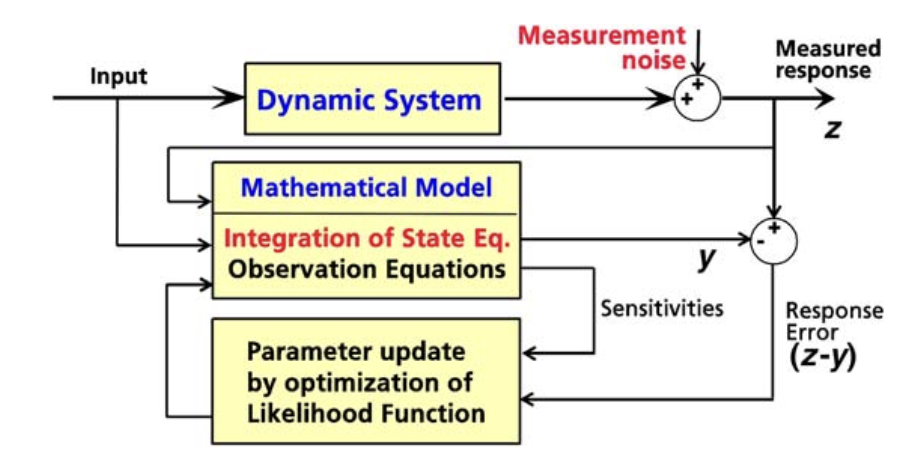
\includegraphics[width=\columnwidth]{images/intro-oem.png}
\caption{Esquema geral do método de erro de saída. Adaptado de~\cite{c2}.}
\label{fig:oem_schematic}
\end{figure}

\begin{figure}[!t]
\centering
\resizebox{\columnwidth}{!}{%
\begin{tikzpicture}[
    node distance=0.9cm,
    block/.style={rectangle, draw=blkEdge, semithick, rounded corners=2pt, minimum width=2.7cm, minimum height=0.7cm, align=center, font=\scriptsize},
    decis/.style={rectangle, draw=blkEdge, semithick, rounded corners=2pt, fill=blkBase, minimum width=2.4cm, minimum height=0.7cm, align=center, font=\scriptsize},
    hi/.style={fill=blkHi, draw=blkHiEdge, thick},
    arrow/.style={-{Stealth[length=2mm]}, semithick, black!62},
    dasharrow/.style={-{Stealth[length=2mm]}, semithick, dashed, black!48},
    lbl/.style={font=\tiny, fill=white, inner sep=1pt, text=black!80}
]

% --- Topo: Parâmetros (esquerda) e Medições (direita) ---
\node[block, fill=blkBase] (theta)
    {$\Theta_j$ -- Parâmetros atuais};

\node[block, fill=blkBase, right=1.5cm of theta] (data)
    {Medições $z(t_k)$\\(sensores)};

% --- Coluna central (entre theta e data) ---
\node[block, hi, below=0.9cm of $(theta.south)!0.5!(data.south)$] (model)
    {Modelo Matemático\\(integração RK4)};

\node[block, fill=blkBase, below=of model] (resid)
    {Erro de saída ponderado\\$\mathbf{W}^{1/2}\big[z(t_k) - y(t_k,\Theta)\big]$};

\node[block, fill=blkBase, below=of resid] (lsq)
    {\textbf{Eq.~\eqref{eq:oem-cost}} -- $\min J(\Theta)$};

\node[decis, below=of lsq] (conv) {Convergiu?};

\node[block, hi, below=of conv] (r2)
    {\textbf{Eq.~\eqref{eq:r2}} -- $R^2$ por canal\\(validação)};

% --- Esquerda: interno lsqnonlin ---
\node[block, fill=blkBase, left=0.5cm of lsq] (jac)
    {\textbf{Eq.~\eqref{eq:sens}} -- Sensibilidades\\$S = \partial y / \partial \Theta$};

\node[block, fill=blkBase, left=0.5cm of resid] (update)
    {\textbf{Eq.~\eqref{eq:update}} -- Atualização\\$\Theta_{j+1} = \Theta_j + \delta$};

% === SETAS ===
\draw[arrow] (theta) |- (model);
\draw[arrow] (model) -- node[lbl, right] {$y(t_k,\Theta)$} (resid);
\draw[arrow] (resid) -- (lsq);
\draw[arrow] (lsq) -- (conv);
\draw[arrow] (conv) -- node[lbl, right] {Sim} (r2);

% Dados → resíduos (desce do topo)
\draw[arrow] (data) |- (resid);

% Interno lsqnonlin
\draw[dasharrow] (lsq) -- (jac);
\draw[dasharrow] (jac) -- (update);

% Não → atualização (contorna pelo lado esquerdo)
\coordinate (aux) at ([xshift=-0.7cm]jac.west);
\draw[arrow] (conv.west) -| node[lbl, near start, above] {Não} (aux) |- (update.west);

% Loop de volta
\draw[arrow] (update) -- (theta);

% Caixa tracejada
\begin{scope}[on background layer]
\node[draw=gray, dashed, rounded corners=4pt, fill=gray!5,
      inner xsep=8pt, inner ysep=8pt,
      fit=(jac)(update),
      label={[font=\tiny, text=gray]above: }] {};
\end{scope}

\end{tikzpicture}%
}
\caption{Ciclo iterativo do método do erro de saída. Adaptado de~\cite{c2}.}
\label{fig:opt_loop}
\end{figure}

O ciclo de integração do modelo para formar o erro de saída, e calcular as sensibilidades e atualizar os parâmetros, repete-se até a convergência, conforme ilustra a Figura~\ref{fig:opt_loop}. Na implementação, as sensibilidades são calculadas por diferenças finitas, a inversa da covariância $\mathbf{R}_\nu^{-1}$ é aproximada pela matriz diagonal fixa de pesos $\mathbf{W} = \mathrm{diag}(1/\sigma_i^2)$, cujos elementos são o inverso da variância de cada canal de saída, e o passo $\delta$ é determinado pelo algoritmo \textit{Trust-Region Reflective}~\cite{c2} da função \texttt{lsqnonlin} do MATLAB, que globaliza o Gauss--Newton e impõe os limites físicos dos parâmetros.

A qualidade do ajuste é avaliada pelo coeficiente de determinação, calculado para cada canal de saída em um segmento de validação que não participa da otimização:
\begin{equation}
R^2 = 1 - \frac{\sum_{k}(z_k - y_k)^2}{\sum_{k}(z_k - \bar{z})^2}
\label{eq:r2}
\end{equation}
onde $\bar{z}$ é a média das medições, e valores próximos de 1 indicam boa aderência entre modelo e dados. Na convergência, a inversa da matriz de informação de Fisher $F$ (Equação~\eqref{eq:gauss-newton}) fornece a covariância das estimativas (limite de Cramér--Rao), de onde se extrai o desvio-padrão relativo de cada parâmetro; valores elevados sinalizam parâmetros pouco observáveis pelos dados~\cite{c2}.

\subsection{Método de Erro de Saída com Multijanelas}

Neste trabalho, a estimação dos parâmetros foi realizada por meio do Método de Erro de Saída (\textit{Output Error Method} -- OEM) com uma estratégia de multijanelas progressivas. Diferentemente do OEM convencional, que integra o modelo ao longo de todo o registro de voo com uma única condição inicial, a abordagem por multijanelas divide cada segmento de dados em janelas temporais menores. No início de cada janela, os estados do modelo são reinicializados com os valores medidos, de modo que os erros de integração não se propagam entre janelas adjacentes. Isso aumenta significativamente a robustez da identificação, pois impede que divergências locais contaminem o restante da simulação.

O processo de identificação é dividido em duas fases sequenciais, conforme ilustrado na Figura~\ref{fig:oem_diagram}:

\begin{itemize}
    \item \textbf{Fase A -- EEM (Equation Error Method):} Os dados de todos os segmentos de treino são concatenados e utilizados em uma formulação algébrica (sem integração numérica). Os parâmetros rotacionais são estimados minimizando o erro entre as derivadas angulares medidas e as calculadas pelo modelo. Esta fase fornece uma estimativa inicial robusta $\Theta_{\text{EEM}}$ para a Fase B.
    \item \textbf{Fase B -- OEM (Output Error Method) Progressivo:} Utilizando como valores iniciais de $\Theta$, os valores de $\Theta_{\text{EEM}}$, o modelo é integrado numericamente com RK4 dentro de cada janela. A duração da janela é progressivamente aumentada, de modo que nas primeiras etapas o otimizador ajusta os parâmetros com menor risco de divergência. A cada estágio, o desempenho é avaliado no segmento de validação, e o conjunto de parâmetros com melhor coeficiente de determinação $R^2$ é selecionado como resultado final $\Theta_{\text{OEM}}$.
\end{itemize}

A função de custo é a mesma do OEM (Equação~\eqref{eq:oem-cost}, com $\mathbf{R}_\nu^{-1} \approx \mathbf{W}$), agora agregando os resíduos ponderados de todas as janelas de todos os segmentos de treino:
\begin{align}
J(\Theta) = \sum_{s=1}^{N_s} \sum_{w=1}^{N_w^{(s)}} \sum_{k \in \mathcal{W}_w^{(s)}} \left\| \mathbf{W}^{1/2} \left[ z(t_k) - y(t_k, \Theta) \right] \right\|^2
\end{align}
onde $N_s$ é o número de segmentos de treino, $N_w^{(s)}$ é o número de janelas no segmento $s$, $\mathcal{W}_w^{(s)}$ são os índices temporais da janela $w$, e $\mathbf{W}^{1/2}$ é a raiz quadrada da matriz de pesos conforme definido anteriormente. As saídas $z$ e $y$ incluem tanto as velocidades angulares $(p, q, r)$ quanto as forças específicas medidas pela IMU $(a_x, a_y, a_z)$.

\begin{figure}[!htbp]
\centering
\resizebox{\columnwidth}{!}{%
\begin{tikzpicture}[
    node distance=0.6cm and 0.4cm,
    block/.style={rectangle, draw=blkEdge, semithick, rounded corners=2pt, fill=blkBase, text width=2.2cm, minimum height=0.7cm, align=center, font=\scriptsize},
    bigblock/.style={rectangle, draw=blkEdge, semithick, rounded corners=2pt, fill=blkBase, text width=2.8cm, minimum height=0.7cm, align=center, font=\scriptsize},
    smallblock/.style={rectangle, draw=blkEdge, semithick, rounded corners=2pt, fill=blkBase, text width=1.4cm, minimum height=0.55cm, align=center, font=\tiny},
    hi/.style={fill=blkHi, draw=blkHiEdge, thick},
    arrow/.style={-{Stealth[length=2mm]}, semithick, black!62},
    every node/.style={font=\scriptsize}
]

% Top: Flight Data
\node[block, fill=blkBase, text width=3cm] (data) {Dados de Voo\\(PWM, $p,q,r$, $\phi,\theta,\psi$, IMU)};

% Segmentation
\node[block, below=0.5cm of data] (seg) {Segmentação Temporal};

% Segments
\node[smallblock, below left=0.5cm and 0.6cm of seg] (s1) {Seg. 1};
\node[smallblock, below=0.5cm of seg] (s2) {Seg. 2};
\node[smallblock, below right=0.5cm and 0.6cm of seg] (sn) {Seg. $N_s$};
\node[smallblock, right=0.3cm of sn, fill=blkBase] (val) {Validação};

% Phase A
\node[bigblock, below=1.2cm of s2, hi, text width=4cm] (eembox) {\textbf{Fase A: EEM}\\Concatena segmentos\\Estimação algébrica $\to \Theta_{\text{EEM}}$};

% Initial parameters
\node[smallblock, left=0.9cm of eembox, text width=1.8cm] (theta0) {$\Theta_0$\\(valores iniciais)};

% Phase B: OEM em tres janelas, todas partindo do mesmo Theta_EEM (paralelo)
\node[block, below=1.5cm of eembox, hi, xshift=-2.8cm, text width=2.3cm] (b1) {\textbf{Fase B.1} $\cdot$ OEM\\janela de 1\,s\\$\Rightarrow \Theta_1$};
\node[block, below=1.5cm of eembox, hi, text width=2.3cm] (b2) {\textbf{Fase B.2} $\cdot$ OEM\\janela de 2\,s\\$\Rightarrow \Theta_2$};
\node[block, below=1.5cm of eembox, hi, xshift=2.8cm, text width=2.3cm] (b3) {\textbf{Fase B.3} $\cdot$ OEM\\janela de 3\,s\\$\Rightarrow \Theta_3$};

% Best selection (below the row)
\node[block, below=1.3cm of b2, hi, text width=3.0cm] (best) {Seleciona melhor $R^2$ na validação\\$\Rightarrow \Theta_{\text{OEM}}$};

% Arrows
\draw[arrow] (data) -- (seg);
\draw[arrow] (seg) -- (s1);
\draw[arrow] (seg) -- (s2);
\draw[arrow] (seg) -- (sn);
\draw[arrow] (seg) -- (val);

\draw[arrow] (s1) -- (eembox);
\draw[arrow] (s2) -- (eembox);
\draw[arrow] (sn) -- (eembox);
\draw[arrow] (theta0) -- (eembox);

% O mesmo Theta_EEM alimenta os tres estagios (paralelo)
\draw[arrow] (eembox.south) -- (b1.north);
\draw[arrow] (eembox.south) -- node[pos=0.6, right, font=\tiny] {$\Theta_{\text{EEM}}$} (b2.north);
\draw[arrow] (eembox.south) -- (b3.north);

% Cada estagio gera um candidato -> selecao
\draw[arrow] (b1.south) -- (best.north);
\draw[arrow] (b2.south) -- (best.north);
\draw[arrow] (b3.south) -- (best.north);

% Validacao (tracejada), afastada dos blocos
\draw[arrow, dashed] (val.east) -- ++(1.4,0) |- (best.east);

\end{tikzpicture}%
}
\caption{Diagrama do processo de identificação. A partir dos valores iniciais {\mathversion{normal}$\Theta_0$}, a Fase~A (EEM algébrico) fornece {\mathversion{normal}$\Theta_{\text{EEM}}$}, que alimenta a Fase~B: o OEM é executado e retorna um {\mathversion{normal}$\Theta_{OEM}$}).}
\label{fig:oem_diagram}
\end{figure}

A reinicialização dos estados no início de cada janela é um aspecto fundamental da abordagem. Dentro de cada janela $w$, o integrador RK4 parte das condições iniciais medidas $z(t_{w,0})$ e propaga os estados até o final da janela. Essa técnica, conhecida como \textit{multiple shooting}, garante que o erro de cada janela dependa apenas da qualidade local dos parâmetros, e não do acúmulo de erros de janelas anteriores.

\section{Metodologia}
\label{sec:metodologia}

A abordagem metodológica deste trabalho é fundamentada na estrutura de identificação de sistemas M4V. As etapas práticas envolveram a coleta de dados de voo no modo quadricóptero por meio de manobras específicas, a determinação de constantes iniciais para o modelo e a implementação do modelo matemático em ambiente de simulação para o processo de identificação.

\subsection{Manobras e Dados para Identificação}

A qualidade da identificação depende diretamente da riqueza dos dados coletados. Para garantir excitação suficiente da dinâmica do modo quadricóptero, foram executadas manobras de voo projetadas para excitar os modos de movimento em torno dos eixos principais: rolagem, arfagem e guinada~\cite{c7},~\cite{c8}. Todas as manobras foram realizadas com a aeronave operando exclusivamente no modo quadricóptero, com o motor de cruzeiro desligado.

As manobras adotadas foram do tipo \textit{doublet}, aplicadas a um eixo de cada vez, em que o comando é deslocado abruptamente em um sentido, mantido por um intervalo $\Delta t_{\text{db}}$, invertido por igual intervalo e retornado ao neutro. Por ser simétrico, o \textit{doublet} concentra a energia da excitação na banda em torno da frequência característica $\omega_n$ do canal a identificar, com energia praticamente nula em frequência zero, o que permite dimensionar a largura do pulso por $\Delta t_{\text{db}} \approx 2{,}3/\omega_n$~\cite{c2},~\cite{c3}. Nos comandos do piloto (RCIN) da Figura~\ref{fig:exc_dataset}, os \textit{doublets} de rolagem e arfagem apresentam largura $\Delta t_{\text{db}} \approx 0{,}4$~s e energia concentrada próximo de $1$~Hz, dentro da banda da dinâmica de taxa. Já a guinada, de menor autoridade de controle e resposta mais lenta, não permitiu ter a mesma variação, resultando em um movimento de \textit{doublet} cerca de cinco vezes mais lento ($\Delta t_{\text{db}} \approx 2{,}0$~s), com energia em torno de $0{,}23$~Hz.

A instrumentação embarcada centraliza-se na controladora de voo Pixhawk 2.4.0 (3DR), que executa o \textit{firmware} ArduPilot e registra em \textit{log} todos os sinais de voo, dos comandos de rádio às saídas de PWM e às medições dos sensores. As grandezas inerciais provêm da IMU integrada à controladora, um sensor InvenSense MPU-6000 que reúne acelerômetro e giroscópio de três eixos amostrados a cerca de $25$~Hz: o giroscópio fornece as velocidades angulares $(p, q, r)$ e o acelerômetro as forças específicas $(a_x, a_y, a_z)$. A atitude não é medida diretamente, mas estimada pelo EKF da controladora a partir do giroscópio, do acelerômetro e do magnetômetro, com o posicionamento apoiado por um receptor GPS u-blox M8.

Os dados foram extraídos diretamente dos logs de voo da aeronave~\cite{c9}. Como os sensores da controladora registram em taxas e instantes distintos, todos os canais foram sincronizados por interpolação em uma grade temporal comum de $10$~Hz ($\Delta t = 0{,}1$~s), como a dinâmica de taxa do quadricóptero concentra-se abaixo de $2$~Hz, essa taxa é cerca de cinco vezes a banda de interesse, o que representa a dinâmica sem perda de informação. Em seguida, aplicou-se um filtro digital de Savitzky--Golay para suprimir o ruído de alta frequência, sobretudo a vibração dos motores, que por ser simétrico não introduz atraso de fase e é aplicado igualmente à entrada e à saída, preservando a relação entrada--saída.

A campanha de voo completa, já reamostrada e filtrada, é apresentada na Figura~\ref{fig:exc_dataset}, cujos painéis reúnem, de cima para baixo, o comando do piloto (RCIN), o comando PWM dos motores, as taxas angulares ($p, q, r$) e as forças específicas do acelerômetro ($a_x, a_y, a_z$). Os dados foram separados em dois grupos de janelas. As janelas de treino (em verde), $\Delta T_1$, $\Delta T_2$ e $\Delta T_3$, que isolam um eixo de cada vez, excitando separadamente a rolagem, a arfagem e a guinada, o que torna a dinâmica de cada canal identificável de forma independente. As janelas de validação (em laranja), $\Delta T_4$ e $\Delta T_5$, as quais contêm movimento composto, com os três eixos excitados simultaneamente, permitindo avaliar o modelo em condições distintas das de treino e evitar o sobreajuste de um único eixo.

\begin{figure}[!htbp]
      \centering
      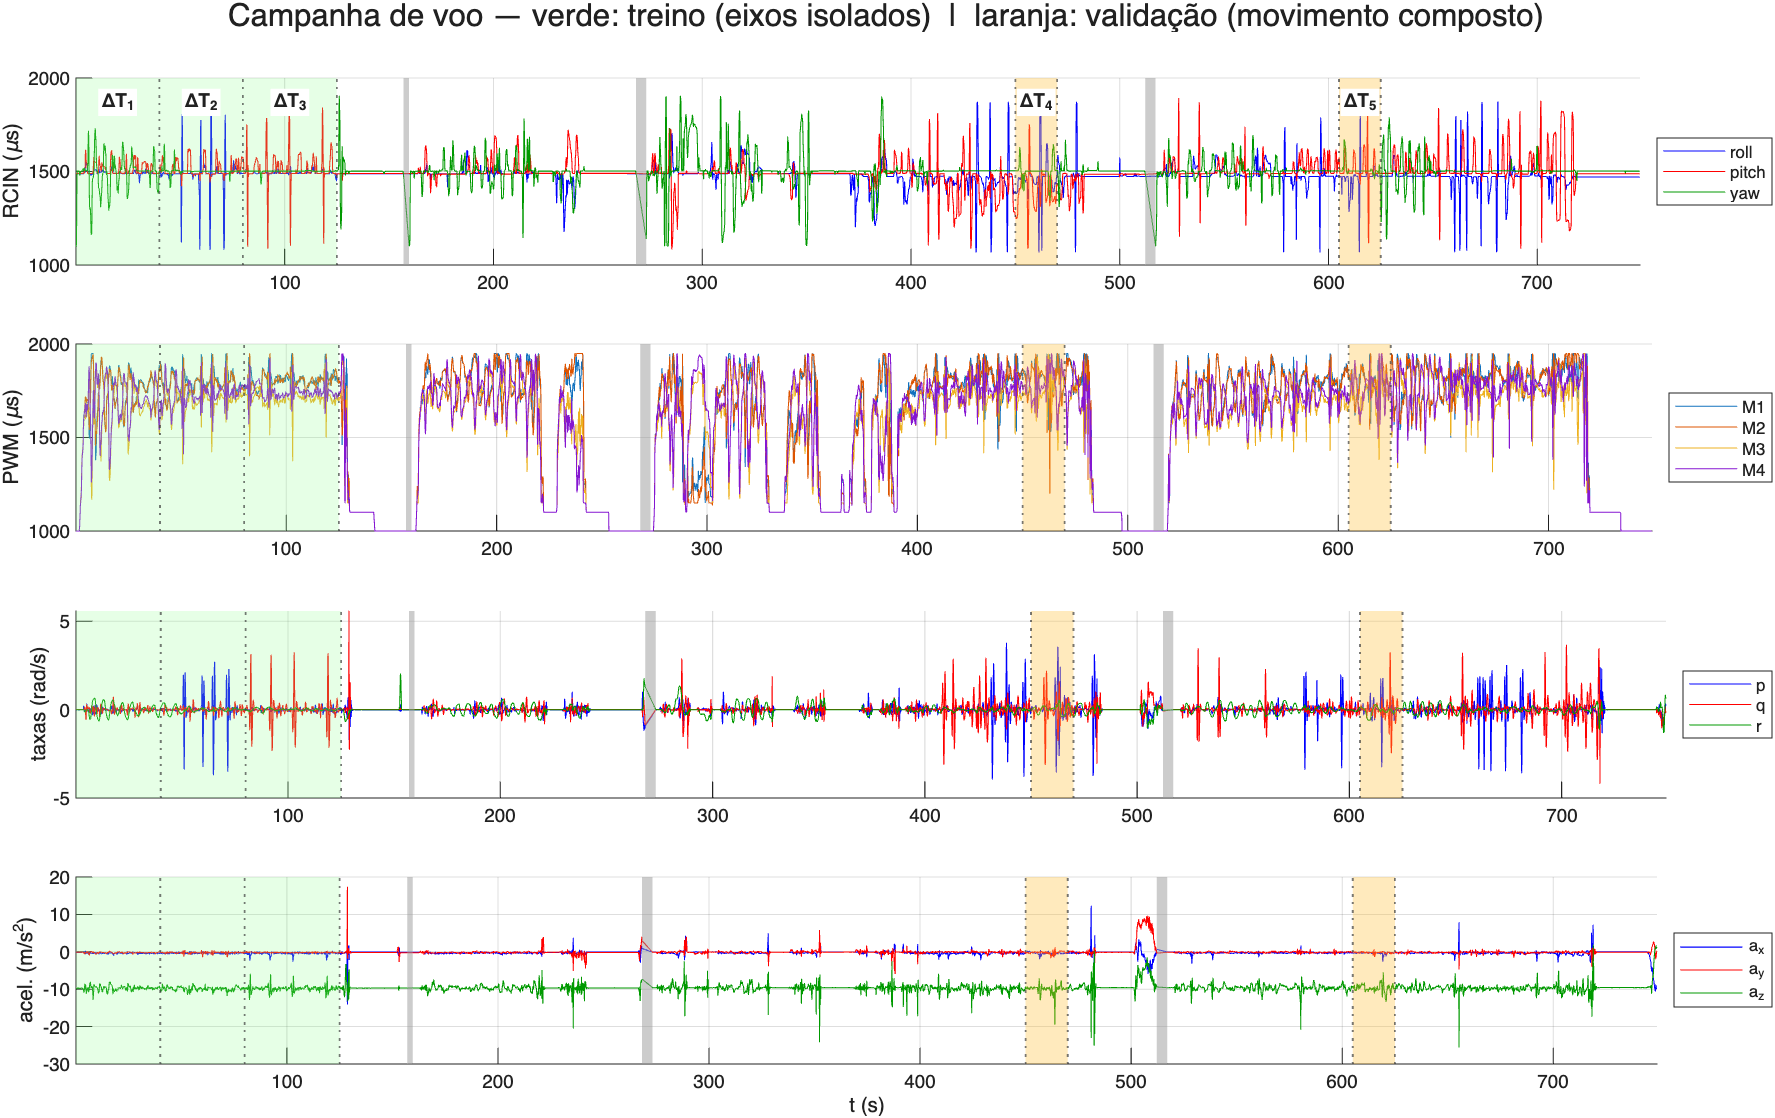
\includegraphics[width=\columnwidth]{exc_dataset.png}
      \caption{Campanha de voo completa: em verde, as janelas de treino ($\Delta T_1$--$\Delta T_3$, eixos isolados); em laranja, as janelas de validação ($\Delta T_4$, $\Delta T_5$, movimento composto).}
      \label{fig:exc_dataset}
\end{figure}

A Figura~\ref{fig:exc_overview} detalha essa cadeia de sinais nos trechos de identificação representativos do voo: o comando do piloto (RCIN) é convertido no PWM efetivamente enviado aos motores (RCOU), que forma a entrada $u$, a qual gera os momentos de controle reconstruídos pela matriz de alocação ($\tau_x, \tau_y, \tau_z$) e, por fim, as taxas angulares de resposta ($p, q, r$), evidenciando o encadeamento entre o comando e a resposta da aeronave que a identificação busca reproduzir.

\begin{figure}[!htbp]
      \centering
      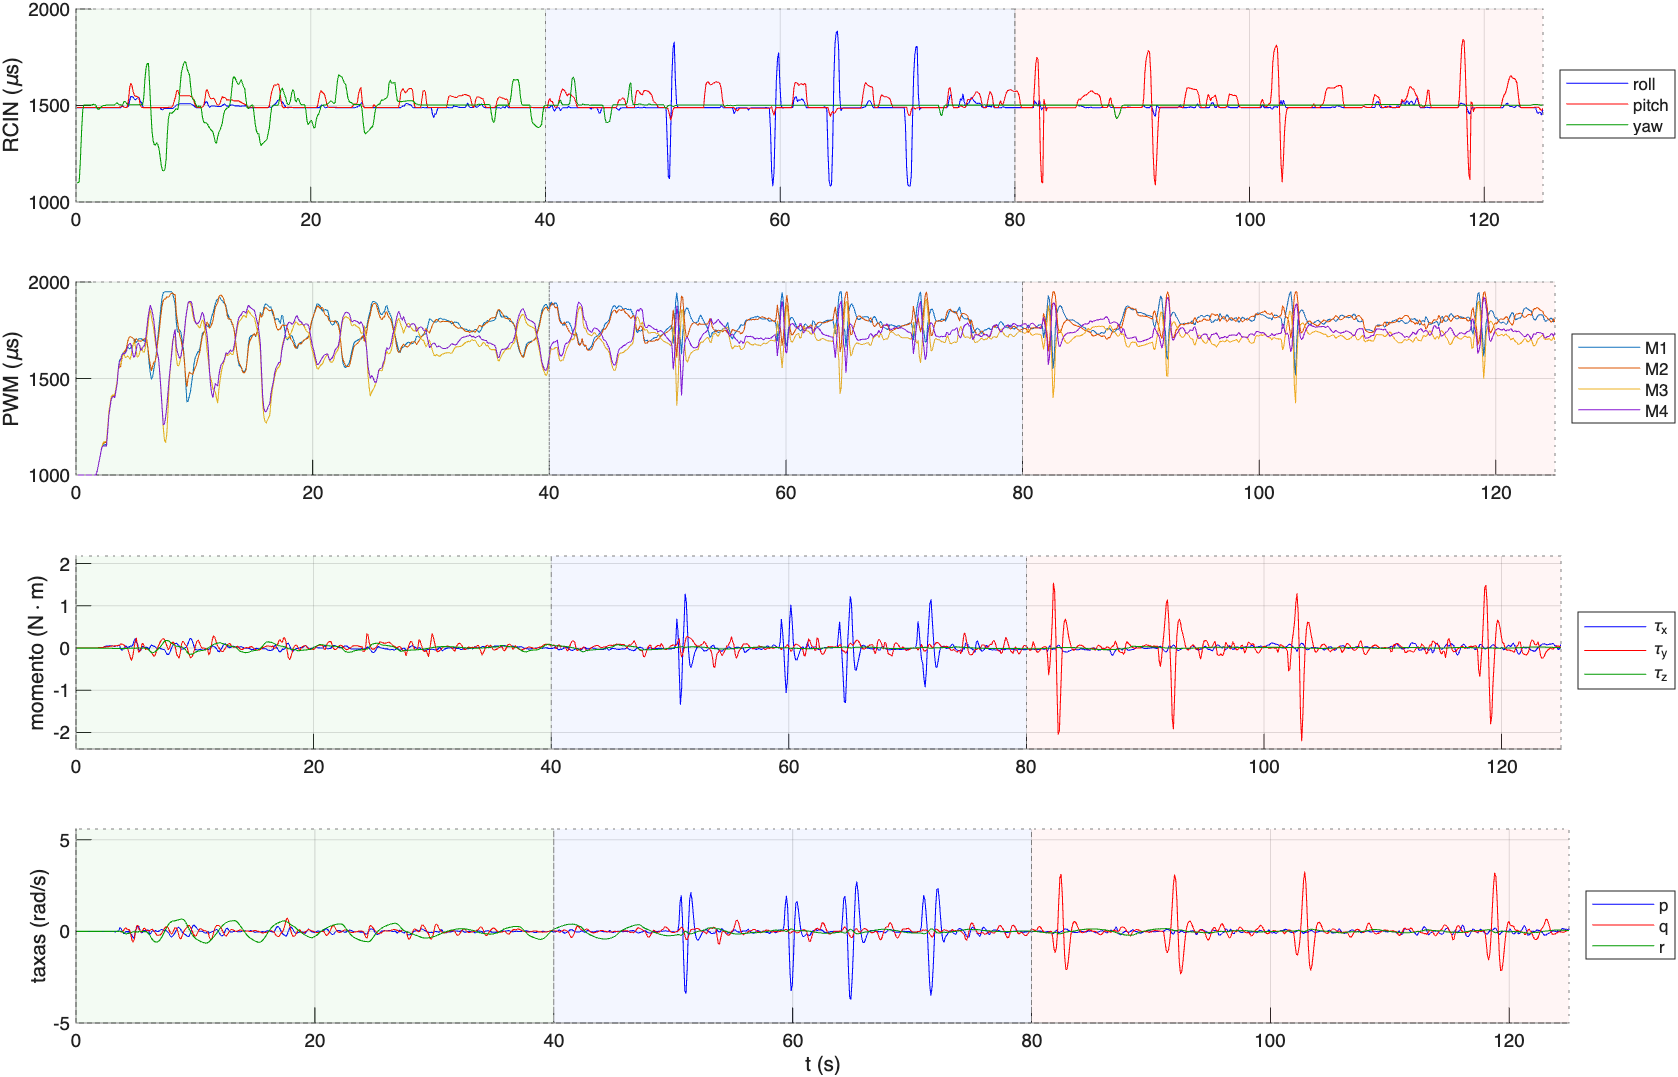
\includegraphics[width=\columnwidth]{exc_overview.png}
      \caption{Cadeia de sinais da excitação em um trecho do voo: comando do piloto (RCIN), PWM dos motores (RCOU), momentos gerados ($\tau_x, \tau_y, \tau_z$) e taxas angulares de resposta ($p, q, r$).}
      \label{fig:exc_overview}
\end{figure}



\pagebreak
Em cada janela, a identificação relaciona a entrada e a saída do sistema:
\begin{sloppypar}
\begin{itemize}
    \item \textbf{Entrada ($u$):} os sinais de Modulação por Largura de Pulso (PWM) enviados aos quatro motores verticais;
    \item \textbf{Saída ($y$):} as velocidades angulares no referencial do corpo, rolagem ($p$), arfagem ($q$) e guinada ($r$), além das forças específicas medidas pela IMU ($a_x$, $a_y$, $a_z$), em rad/s e m/s$^2$, respectivamente.
\end{itemize}
\end{sloppypar}

\subsection{Constantes Fixas do Modelo}
\begin{sloppypar}
As constantes iniciais do modelo foram obtidas por meio de medições físicas da aeronave e dos ensaios em bancada do modelo do motor. As distâncias entre cada rotor e o centro de gravidade, que definem os braços de momento da matriz de alocação, são apresentadas na Figura~\ref{fig:bracos}, e os principais valores iniciais são reunidos na Tabela~\ref{tab:const_iniciais}.
\end{sloppypar}

\begin{figure}[!htbp]
      \centering
      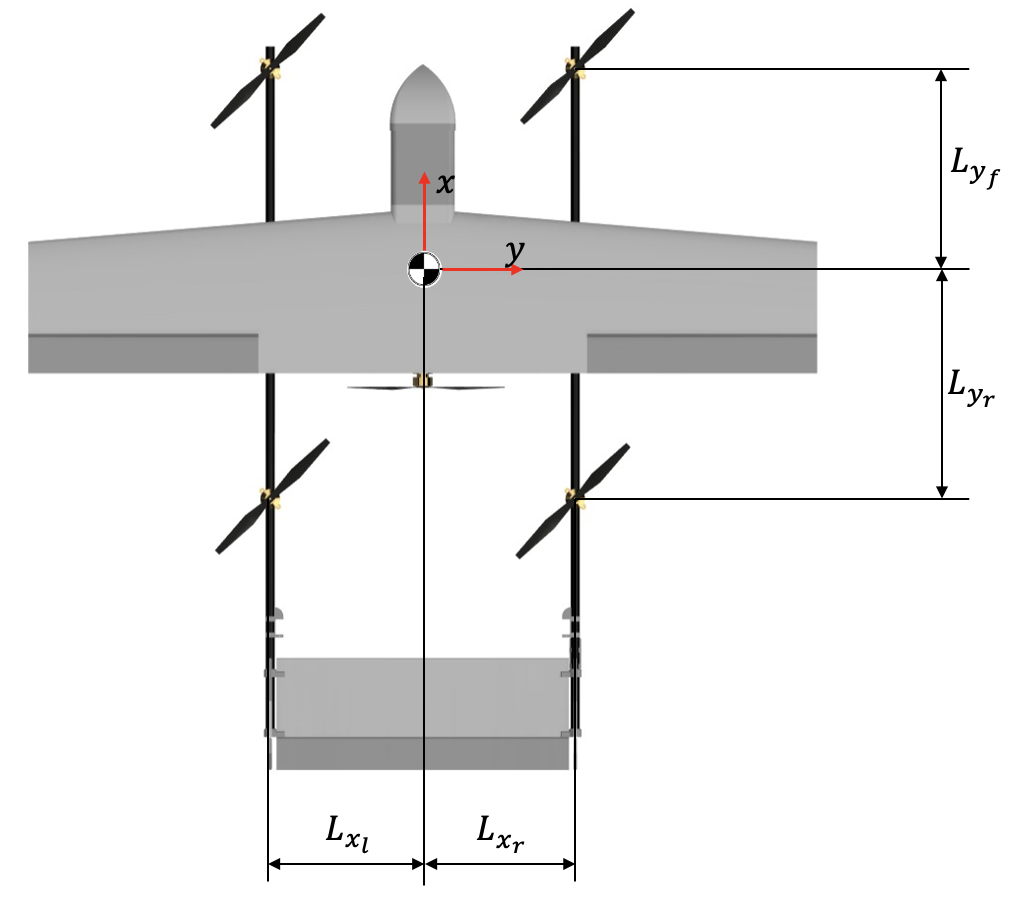
\includegraphics[width=0.8\columnwidth]{bracos.png}
      \caption{Distâncias entre os motores e o CG.}
      \label{fig:bracos}
\end{figure}

\begin{table*}[!htbp]
\caption{Constantes fixas do modelo.}
\label{tab:const_iniciais}
\centering
\begin{tabular}{llccl}
\toprule
\textbf{Constante} & \textbf{Descrição} & \textbf{Valor} & \textbf{Unidade} & \textbf{Modo de obtenção} \\
\midrule
$L_{x_l} = L_{x_r}$ & Braço lateral do CG aos rotores (esquerdo e direito) & 0,232 & m & Medição física \\
$L_{y_f}$ & Braço longitudinal do CG aos rotores dianteiros & 0,330 & m & Medição física \\
$L_{y_r}$ & Braço longitudinal do CG aos rotores traseiros & 0,323 & m & Medição física \\
$r_{\mathrm{imu}_x}$ & Deslocamento longitudinal da IMU em relação ao CG & 0,10 & m & Medição física \\
$r_{\mathrm{imu}_z}$ & Deslocamento vertical da IMU em relação ao CG & 0,02 & m & Medição física \\
$c_{T_0}$ & Coeficiente de empuxo do rotor inicial & $1{,}76\times10^{-7}$ & N/RPM$^2$ & Ensaio em bancada \\
$c_{M_0}$ & Coeficiente de contra-torque do rotor inicial & $5{,}04\times10^{-9}$ & N$\cdot$m/RPM$^2$ & Ensaio em bancada \\
$m$ & Massa total da aeronave & 1,993 & kg & Medição física com balança \\
\bottomrule
\end{tabular}
\end{table*}

Substituindo na Equação~\eqref{eq:aloca} as distâncias medidas e a razão entre os coeficientes de bancada $c_M/c_T = 0{,}0286$~m, a matriz de alocação inicial obtida assume a forma numérica:
\begin{equation}
\mathbf{B_0}=
\begin{bmatrix}
1 & 1 & 1 & 1 \\
-0{,}232 & 0{,}232 & 0{,}232 & -0{,}232 \\
0{,}330 & -0{,}323 & 0{,}330 & -0{,}323 \\
0{,}0286 & 0{,}0286 & -0{,}0286 & -0{,}0286
\end{bmatrix}
\label{eq:aloca_num}
\end{equation}

A última linha, associada à guinada, é cerca de uma ordem de grandeza menor que as de rolagem e arfagem, o que antecipa a menor autoridade de controle e a menor observabilidade desse eixo na identificação.

Também foi medido o desalinhamento da IMU em relação ao centro de gravidade, apresentado na Figura~\ref{fig:imu_offset}, necessário para relacionar as forças específicas registradas pelo sensor com a dinâmica do centro de gravidade.

\begin{figure}[!htbp]
      \centering
      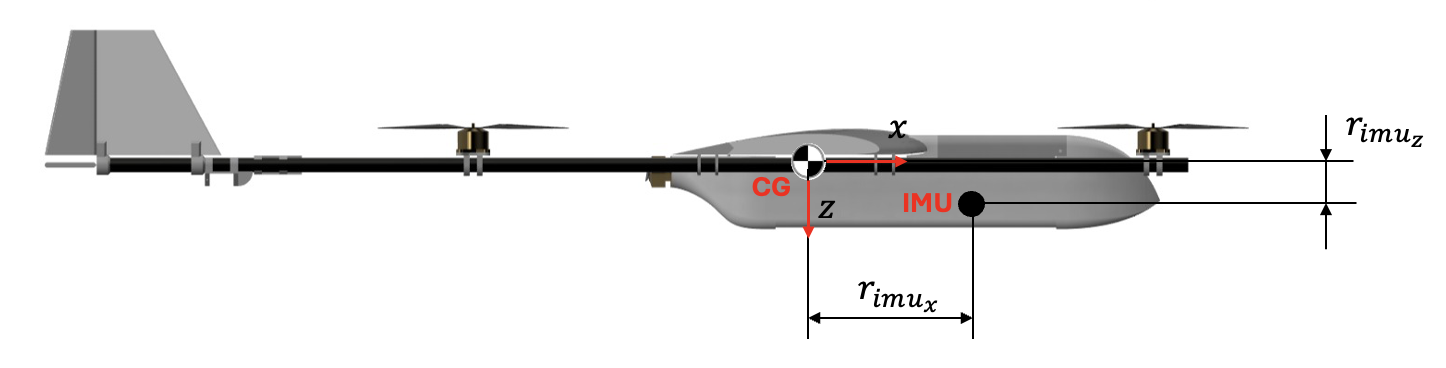
\includegraphics[width=\columnwidth]{displacement.png}
      \caption{Desalinhamento da IMU em relação ao CG.}
      \label{fig:imu_offset}
\end{figure}

Os momentos de inércia iniciais foram estimados a partir das propriedades de massa de um modelo tridimensional (CAD, \textit{Computer-Aided Design}) da aeronave, elaborado no \textit{software} SolidWorks, sendo posteriormente refinados pelo processo de identificação.

\subsection{Simulação Dinâmica do Modelo}

O conjunto de equações diferenciais não-lineares que descreve a dinâmica do modo quadricóptero foi implementado em MATLAB. O modelo foi estruturado em blocos que calculam as forças e momentos de propulsão a partir das curvas de bancada, aplicam o arrasto aerodinâmico, integram as equações de movimento rotacional e translacional (via Runge-Kutta de 4\textordfeminine\ ordem) e propagam a cinemática de Euler, conforme o diagrama da Figura~\ref{fig:model_diagram}.

A simulação constitui o elemento central do método de estimação: ela gera a resposta prevista do modelo ($y$) para uma dada entrada de controle. Essa resposta é comparada com a resposta real da aeronave ($z$) para formar o vetor de resíduos que o algoritmo de otimização minimiza.

\section{Resultados e Discussões}
\label{sec:resultados}

A aplicação do método dos mínimos quadrados não-lineares aos dados de voo no modo quadricóptero permitiu a estimação dos parâmetros do modelo dinâmico.

\subsection{Resultado da Estimação dos Parâmetros}

O processo de otimização convergiu para o conjunto final de parâmetros $\Theta_{\text{OEM}}$, composto pelos momentos de inércia, pelos coeficientes de empuxo e de contra-torque de cada motor e pelos coeficientes de amortecimento rotacional (Equação~\eqref{eq:theta}). Os valores iniciais ($\Theta_0$) e os parâmetros estimados são apresentados nas Tabelas~\ref{tab:param_inercia},~\ref{tab:param_motor},~\ref{tab:param_motor_cm} e~\ref{tab:param_rot}. Os momentos de inércia $J_{xx}$ e $J_{yy}$ sobem cerca de 8,6\,\% e 16,6\,\% em relação ao modelo tridimensional (CAD), respectivamente, refletindo as particularidades da configuração VTOL híbrida, em que a presença das superfícies aerodinâmicas e do motor traseiro influencia a distribuição de massa mesmo quando inativos no modo quadricóptero.

\begin{table}[!htbp]
\caption{Momentos e produtos de inércia.}
\label{tab:param_inercia}
\centering
\small
\begin{tabular}{lccccc}
\toprule
 & \multicolumn{2}{c}{\textbf{\boldmath$\Theta_0$}} & \multicolumn{2}{c}{\textbf{\boldmath$\Theta_{\text{OEM}}$}} & \\
\cmidrule(lr){2-3}\cmidrule(lr){4-5}
\textbf{Parâmetro} & \textbf{Valor} & \textbf{CRB} & \textbf{Valor} & \textbf{CRB} & \textbf{Unidade} \\
\midrule
$J_{xx}$ & 0,0432 & 1,9\% & 0,0469 & 1,8\% & kg$\cdot$m$^2$ \\
$J_{yy}$ & 0,0844 & 1,7\% & 0,0984 & 1,7\% & kg$\cdot$m$^2$ \\
$J_{zz}$ & 0,1262 & 19,3\% & 0,1453 & 19,2\% & kg$\cdot$m$^2$ \\
$J_{xz}$ & 0,00157 & 70,3\% & 0,00261 & 30,4\% & kg$\cdot$m$^2$ \\
\bottomrule
\end{tabular}
\end{table}

\begin{table}[!htbp]
\caption{Coeficientes de empuxo $c_{T_i}$ ($\times 10^{-7}$~N/RPM$^2$) por motor.}
\label{tab:param_motor}
\centering
\small
\begin{tabular}{lcccc}
\toprule
 & \multicolumn{2}{c}{\textbf{\boldmath$\Theta_0$}} & \multicolumn{2}{c}{\textbf{\boldmath$\Theta_{\text{OEM}}$}} \\
\cmidrule(lr){2-3}\cmidrule(lr){4-5}
\textbf{Parâmetro} & \textbf{Valor} & \textbf{CRB} & \textbf{Valor} & \textbf{CRB} \\
\midrule
$c_{T_1}$ & 1,76 & 1,2\% & 1,87 & 1,1\% \\
$c_{T_2}$ & 1,76 & 1,2\% & 1,86 & 1,1\% \\
$c_{T_3}$ & 1,76 & 1,3\% & 1,86 & 1,3\% \\
$c_{T_4}$ & 1,76 & 1,2\% & 1,89 & 1,2\% \\
\bottomrule
\end{tabular}
\end{table}

\begin{table}[!htbp]
\caption{Coeficientes de contra-torque $c_{M_i}$ ($\times 10^{-9}$~N$\cdot$m/RPM$^2$) por motor.}
\label{tab:param_motor_cm}
\centering
\small
\begin{tabular}{lcccc}
\toprule
 & \multicolumn{2}{c}{\textbf{\boldmath$\Theta_0$}} & \multicolumn{2}{c}{\textbf{\boldmath$\Theta_{\text{OEM}}$}} \\
\cmidrule(lr){2-3}\cmidrule(lr){4-5}
\textbf{Parâmetro} & \textbf{Valor} & \textbf{CRB} & \textbf{Valor} & \textbf{CRB} \\
\midrule
$c_{M_1}$ & 5,04 & 47,4\% & 3,38 & 26,1\% \\
$c_{M_2}$ & 5,04 & 54,7\% & 3,16 & 25,5\% \\
$c_{M_3}$ & 5,04 & 42,9\% & 3,92 & 29,5\% \\
$c_{M_4}$ & 5,04 & 48,1\% & 3,47 & 27,3\% \\
\bottomrule
\end{tabular}
\end{table}

\begin{table}[!htbp]
\caption{Coeficientes de amortecimento rotacional.}
\label{tab:param_rot}
\centering
\small
\begin{tabular}{lccccc}
\toprule
 & \multicolumn{2}{c}{\textbf{\boldmath$\Theta_0$}} & \multicolumn{2}{c}{\textbf{\boldmath$\Theta_{\text{OEM}}$}} & \\
\cmidrule(lr){2-3}\cmidrule(lr){4-5}
\textbf{Parâmetro} & \textbf{Valor} & \textbf{CRB} & \textbf{Valor} & \textbf{CRB} & \textbf{Unidade} \\
\midrule
$c_p$ & 0,5 & 32,9\% & 6,85 & 2,3\% & s$^{-1}$ \\
$c_q$ & 0,5 & 22,5\% & 4,68 & 2,2\% & s$^{-1}$ \\
$c_r$ & 0,5 & 7,7\% & 0,81 & 3,6\% & s$^{-1}$ \\
\bottomrule
\end{tabular}
\end{table}

Os coeficientes de empuxo $c_{T_i}$ sobem para aproximadamente $1{,}87\times10^{-7}$~N/RPM$^2$, corrigindo a subestimação do EEM, enquanto os de contra-torque $c_{M_i}$ caem cerca de 30\,\% em relação à bancada, refletindo a sobrestimação do torque medido em ensaio estático. Entre os amortecimentos, $c_r$ (guinada) é o menor, coerente com a baixa autoridade e a menor observabilidade desse eixo, os coeficientes de contra-torque $c_{M_i}$ e o produto de inércia $J_{xz}$, associados à guinada, apresentam os maiores desvios relativos (acima de 20\,\%, pelo limite de Cramér--Rao), ao passo que $J_{xx}$, $J_{yy}$, $c_{T_i}$ e os amortecimentos ficam abaixo de 5\,\%.

\subsection{Validação}
A validação do modelo identificado foi realizada comparando a resposta simulada com um conjunto de dados de voo no modo quadricóptero não utilizado no processo de estimação. As Figuras~\ref{fig:pqr_val} e~\ref{fig:acc_val} apresentam, para as velocidades angulares e as forças específicas, a comparação entre os dados medidos e as respostas dos modelos inicial com $\Theta_0$, do EEM e do OEM final, evidenciando a melhora progressiva da estimação.

\begin{figure}[!htbp]
    \centering
    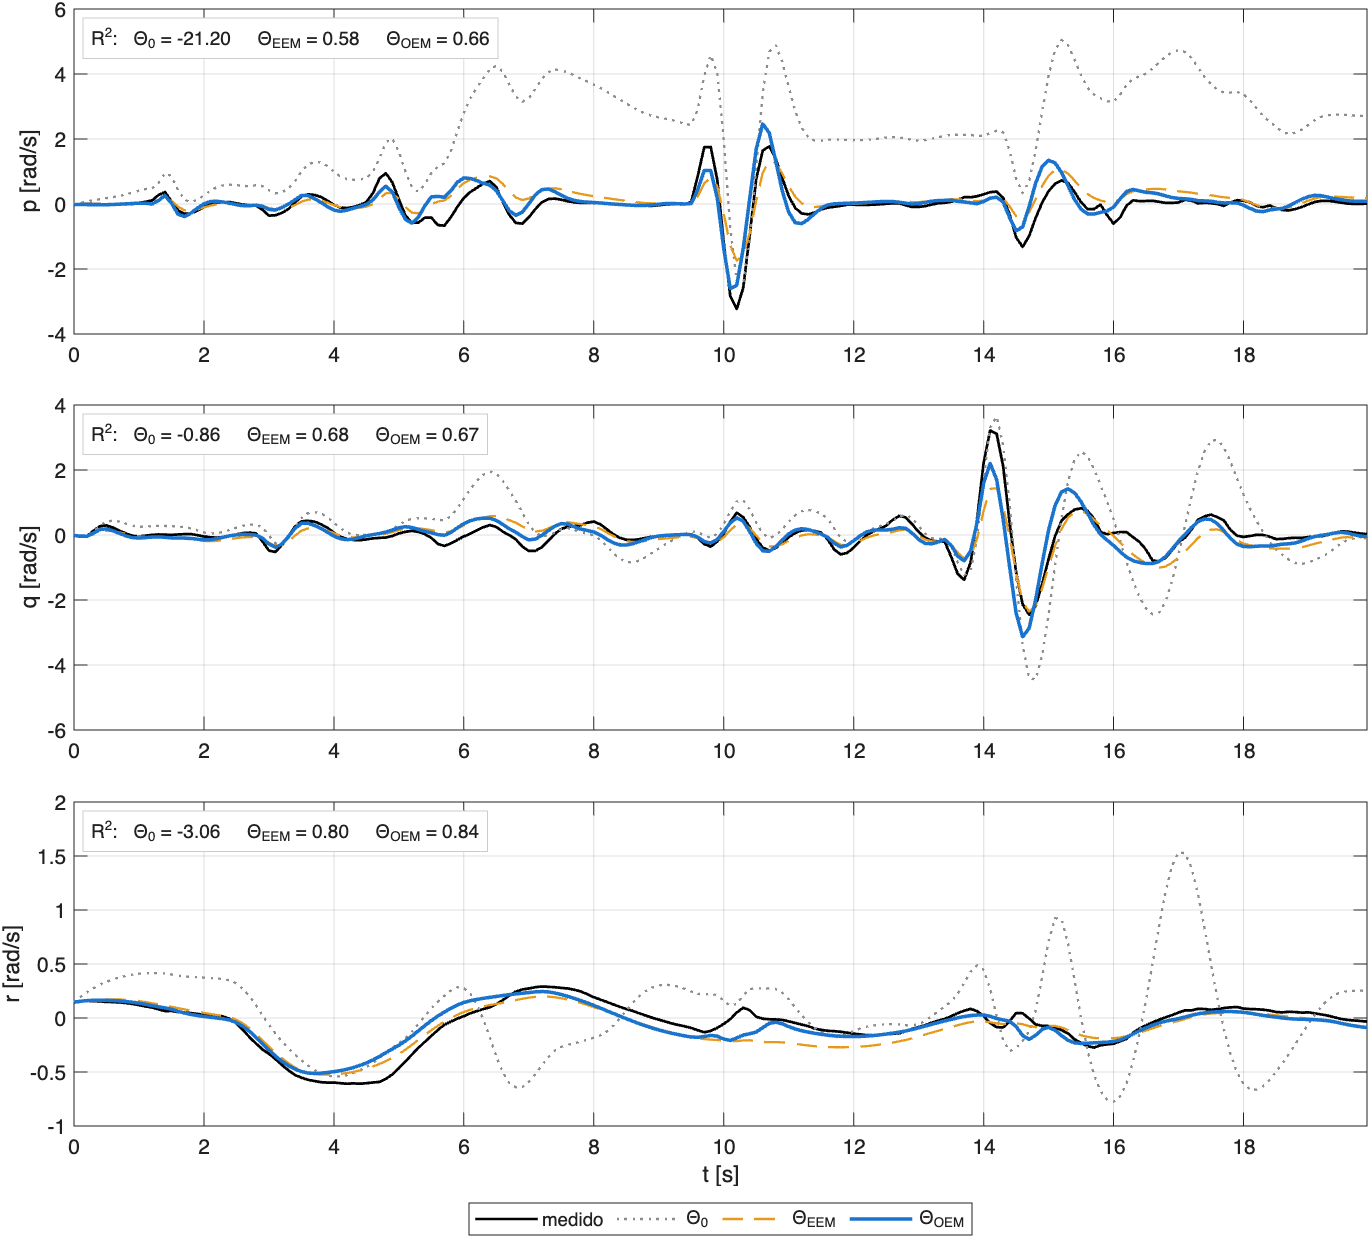
\includegraphics[width=\columnwidth]{id_comp_rates.png}
    \caption{Velocidades angulares: comparação das respostas dos modelos {\mathversion{normal}$\Theta_0$}, {\mathversion{normal}$\Theta_{\text{EEM}}$} e {\mathversion{normal}$\Theta_{\text{OEM}}$} às medições, no segmento de validação.}
    \label{fig:pqr_val}
\end{figure}

\begin{figure}[!htbp]
    \centering
    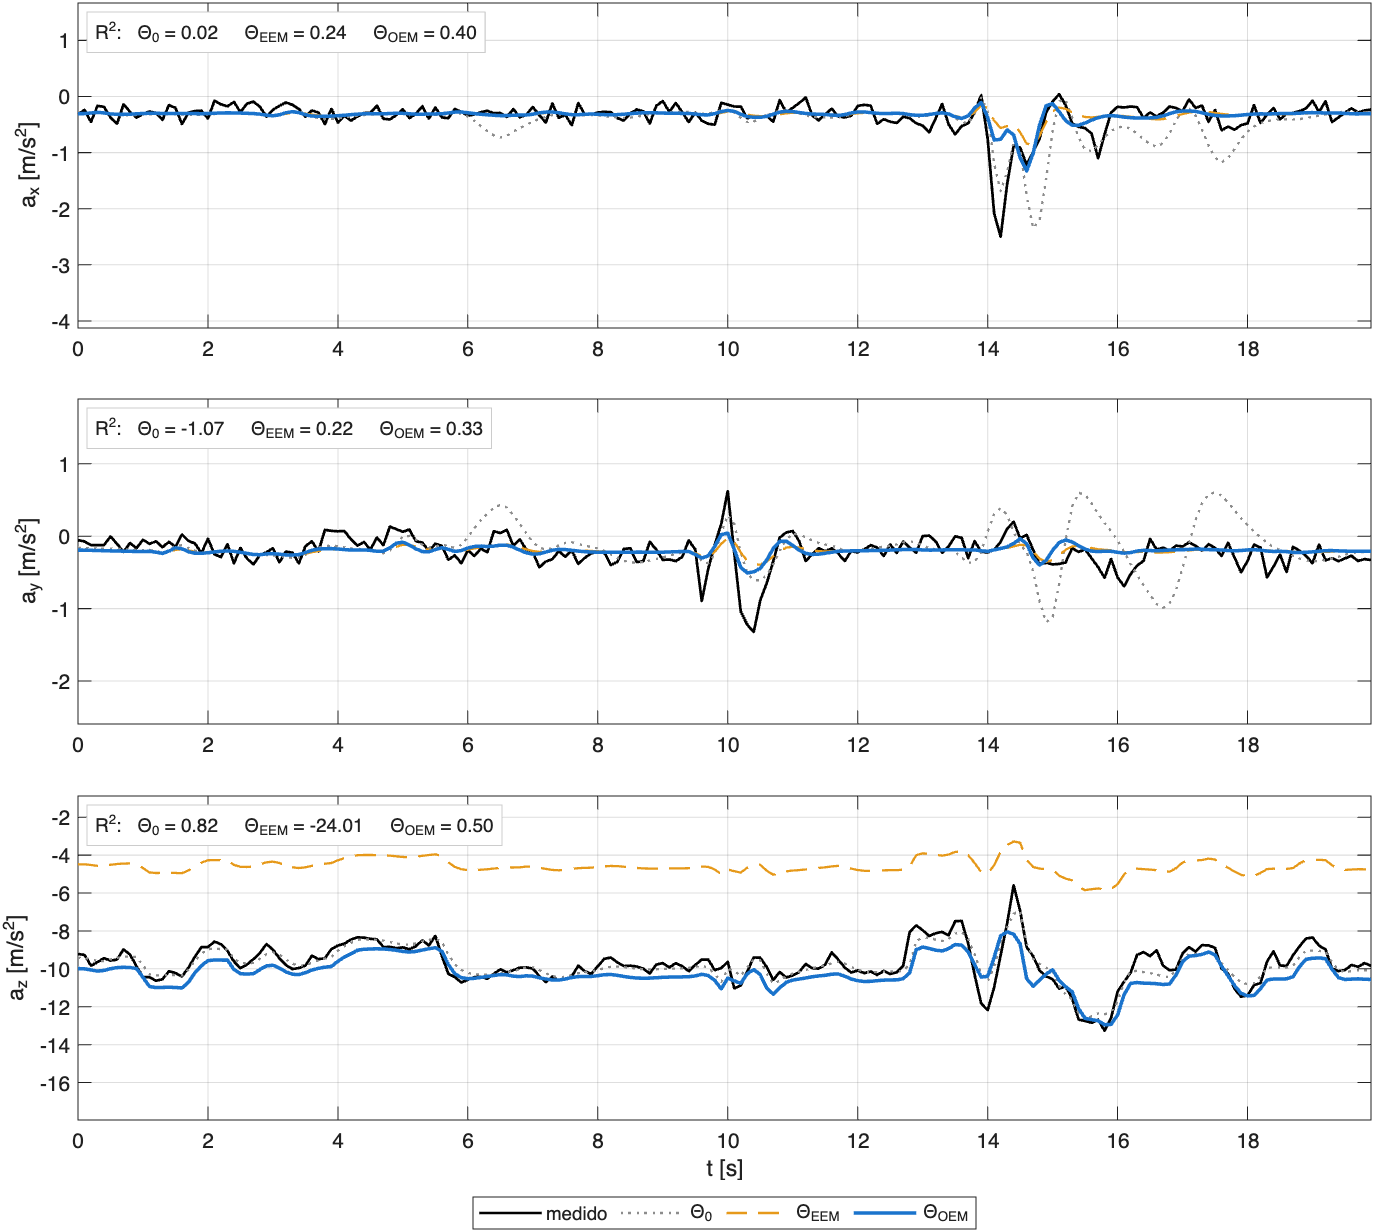
\includegraphics[width=\columnwidth]{id_comp_acc.png}
    \caption{Acelerações (força específica da IMU): comparação das respostas dos modelos {\mathversion{normal}$\Theta_0$}, {\mathversion{normal}$\Theta_{\text{EEM}}$} e {\mathversion{normal}$\Theta_{\text{OEM}}$} às medições, no segmento de validação.}
    \label{fig:acc_val}
\end{figure}

O coeficiente de determinação $R^2$ obtido em cada canal no segmento de validação, para os modelos inicial $\Theta_0$ e final $\Theta_{\text{OEM}}$, é apresentado na Tabela~\ref{tab:r2_val}. O modelo inicial apresenta $R^2$ fortemente negativo nas taxas (chegando a $-21{,}2$ em $p$), indicando que, sem os parâmetros estimados, a simulação diverge das medições. Já no modelo final, as velocidades angulares apresentam boa aderência ($R^2$ entre 0,66 e 0,84), com a guinada ($r$) o melhor canal; as forças específicas são reproduzidas de forma moderada ($R^2$ entre 0,33 e 0,50), refletindo os limites do modelo de sensor para as acelerações.

\begin{table}[!htbp]
\caption{Coeficiente de determinação $R^2$ por canal no segmento de validação, para os modelos inicial {\mathversion{normal}$\Theta_0$} e final {\mathversion{normal}$\Theta_{\text{OEM}}$}.}
\label{tab:r2_val}
\centering
\begin{tabular}{lcccccc}
\toprule
\textbf{Modelo} & $p$ & $q$ & $r$ & $a_x$ & $a_y$ & $a_z$ \\
\midrule
$\Theta_0$ (inicial) & $-21{,}2$ & $-0{,}86$ & $-3{,}06$ & $0{,}02$ & $-1{,}07$ & $0{,}82$ \\
$\Theta_{\text{OEM}}$ (final) & $0{,}66$ & $0{,}67$ & $0{,}84$ & $0{,}40$ & $0{,}33$ & $0{,}50$ \\
\bottomrule
\end{tabular}
\end{table}

Os resultados demonstram boa aderência entre o modelo identificado e os dados reais, indicando que o modelo captura adequadamente a dinâmica do modo quadricóptero, incluindo os efeitos de acoplamento e as assimetrias decorrentes da configuração VTOL híbrida. Essa validação confirma que o modelo é adequado para servir de base ao projeto de controladores para as fases de decolagem e pouso vertical.

\section{Conclusão}
\label{sec:conclusao}

Este trabalho apresentou a identificação do modelo dinâmico do modo quadricóptero de um VANT VTOL de configuração híbrida, levando em consideração as particularidades geométricas e inerciais decorrentes da presença de superfícies aerodinâmicas e motor de cruzeiro na aeronave. Utilizando a metodologia M4V e o método de erro de saída com multijanelas progressivas, foi possível estimar os parâmetros de um modelo não-linear a partir de dados de voo reais.

A partir de constantes iniciais obtidas por medições físicas e ensaios de bancada, o modelo físico do motor e a matriz de alocação reconstruíram os esforços de controle diretamente dos comandos PWM, enquanto os momentos de inércia $J_{xx}$ e $J_{yy}$, os coeficientes de empuxo e de contra-torque de cada motor e os coeficientes de amortecimento rotacional foram refinados pela otimização. A validação com dados de voo independentes apresentou coeficientes de determinação de 0,66, 0,67 e 0,84 nas taxas de rolagem, arfagem e guinada, confirmando a capacidade preditiva do modelo. A análise de Cramér--Rao aponta a guinada como o eixo de menor observabilidade, com os coeficientes de contra-torque entre os parâmetros menos bem determinados, em coerência com a baixa autoridade de controle desse eixo na configuração H-frame.

O modelo identificado constitui a base para o desenvolvimento de algoritmos de controle e de um piloto automático (PA) para as fases de decolagem e pouso vertical autônomo. Trabalhos futuros incluem o projeto dos controladores de atitude e altitude, bem como a extensão da identificação para os modos de transição e asa fixa.

\section*{Agradecimentos}
Os autores agradecem ao Instituto Tecnológico de Aeronáutica (ITA) pelo apoio ao desenvolvimento deste trabalho.

\begin{thebibliography}{99}

\bibitem{c1} V. Klein and E. A. Morelli, \textit{Aircraft System Identification: Theory and Practice}. Reston, VA, USA: AIAA, 2006, doi: 10.2514/4.861505.

\bibitem{c2} R. V. Jategaonkar, \textit{Flight Vehicle System Identification: A Time Domain Methodology}. Reston, VA, USA: AIAA, 2006, ISBN: 1-56347-836-6.

\bibitem{c3} M. B. Tischler and R. K. Remple, \textit{Aircraft and Rotorcraft System Identification}, 2nd ed. Reston, VA, USA: AIAA, 2012, doi: 10.2514/4.868207.

\bibitem{c4} N. V. Hoffer, C. Coopmans, A. M. Jensen, and Y. Chen, ``A survey and categorization of small low-cost unmanned aerial vehicle system identification,'' \textit{J. Intell. Robot. Syst.}, vol. 74, no. 1--2, pp. 129--145, 2014, doi: 10.1007/s10846-013-9931-6.

\bibitem{c5} O. Arifianto and M. Farhood, ``Development and modeling of a low-cost unmanned aerial vehicle research platform,'' \textit{J. Intell. Robot. Syst.}, vol. 80, no. 1, pp. 139--164, Oct. 2015, doi: 10.1007/s10846-014-0145-3.

\bibitem{c7} D. J. Grymin and M. Farhood, ``Two-step system identification and trajectory tracking control of a small fixed-wing UAV,'' \textit{J. Intell. Robot. Syst.}, vol. 83, no. 1, pp. 105--131, 2016, doi: 10.1007/s10846-015-0298-8.

\bibitem{c8} S. Bouabdallah and R. Siegwart, ``Full control of a quadrotor,'' in \textit{Proc. IEEE/RSJ Int. Conf. Intell. Robots Syst. (IROS)}, Oct. 2007, pp. 153--158, doi: 10.1109/IROS.2007.4399042.

\bibitem{c9} D. Mellinger and V. Kumar, ``Minimum snap trajectory generation and control for quadrotors,'' in \textit{Proc. IEEE Int. Conf. Robot. Autom. (ICRA)}, May 2011, pp. 2520--2525, doi: 10.1109/ICRA.2011.5980409.

\bibitem{c11} B. P. Graesdal, ``Full nonlinear system identification for a vertical-takeoff-and-landing unmanned aerial vehicle,'' M.S. thesis, Dept. Eng. Cybern., Norwegian Univ. Sci. Technol. (NTNU), Trondheim, Norway, 2022.

\bibitem{c12} L. E. Hale, M. Patil, and C. J. Roy, ``Aerodynamic parameter identification and uncertainty quantification for small unmanned aircraft,'' \textit{J. Guid. Control Dyn.}, vol. 40, no. 3, pp. 680--691, 2017, doi: 10.2514/1.G000582.

\bibitem{cBeard} R. W. Beard and T. W. McLain, \textit{Small Unmanned Aircraft: Theory and Practice}. Princeton, NJ, USA: Princeton Univ. Press, 2012, ISBN: 978-0-691-14921-9.

\bibitem{c13} Q. Quan, \textit{Introduction to Multicopter Design and Control}. Singapore: Springer, 2017, doi: 10.1007/978-981-10-3382-7.

\end{thebibliography}

\EOD

\end{document}
